\documentclass[11pt,a4paper,twoside]{report}
\usepackage{fullpage}
\usepackage{graphicx}
\usepackage{setspace}
\usepackage{caption}
\usepackage{subcaption}
\usepackage{hyperref}
\usepackage{tikz}
\usepackage{pgfgantt}
\usepackage{lscape}
\usepackage{appendix}
\usepackage{fancyhdr}
\usepackage[utf8]{inputenc}
\usepackage[nottoc,numbib]{tocbibind}
\usetikzlibrary{shapes,arrows}
\onehalfspacing
\hypersetup{
  colorlinks=false,
  pdfborder={0 0 0},
}
\pagestyle{fancy}
\fancyhead[LO,RE]{\thepage}
\fancyfoot{}
\setcounter{tocdepth}{1}

\begin{document}

\begin{titlepage}
  \vspace*{\fill}
  \begin{center}
    {\Huge Assisted navigation of audio in radio production using
      visualisation}\\[1cm]
    {\Large Christopher M. Baume}\\[1cm]
    {\large Submitted for the degree of\\Doctor of Philosophy\\from the\\
      University of Surrey}\\[1cm]
    \begin{center}
      \includegraphics[width=6cm]{figs/surrey-logo.png}
    \end{center}
    \\[1cm]
    {\small Centre for Vision, Speech and Signal Processing,\\
      Faculty of Engineering and Physical Sciences,\\
      University of Surrey,\\
      Guildford, Surrey GU2 7XH, U.K.}
  \end{center}
  \vspace*{\fill}
\end{titlepage}

% !TeX root = main.tex
\chapter*{Abstract}

Radio production is a creative pursuit that uses sound to inform, educate and entertain an audience. Radio producers
use audio editing tools to visually select, re-arrange and assemble sound recordings into programmes. However, current
tools represent audio using waveform visualizations that display limited information about the sound.

Semantic audio analysis can be used to extract useful information from audio recordings, including when people are
speaking and what they are saying. This thesis investigates how such information can be applied to create
semantic audio tools that improve the radio production process.

An initial ethnographic study of radio production at the BBC reveals that producers use textual representations and
paper transcripts to interact with audio, and waveforms to edit programmes. Based on these findings, three
methods for improving radio production are developed and evaluated, which form the primary contribution of this thesis.

Audio visualizations can be enhanced by mapping semantic audio features to colour, but this approach had not been
formally tested. We show that with an enhanced audio waveform, a typical radio production task can be completed faster,
with less effort and with greater accuracy than a normal waveform.

Speech recordings can be represented and edited using transcripts, but this approach had not been formally evaluated
for radio production. By developing and testing a semantic speech editor, we show that automatically-generated
transcripts can be used to semantically edit speech in a professional radio production context, and identify
requirements for annotation, collaboration, portability and listening.

Finally, we present a novel approach for editing audio on paper that combines semantic speech editing with a digital
pen interface. Through a user study with radio producers, we compare the relative benefits of semantic speech editing
using paper and screen interfaces. We find that paper is better for simple edits of familiar audio with accurate
transcripts.
%We also gain insights into the effect of transcription errors and the reasons for listening.



% !TeX root = main.tex
\chapter*{Acknowledgements}
This is the acknowledgements

% SUPERVISORS
% Prof. Mark Plumbley
% Prof. David Frohlich
% Dr. Janko Calic
% Dr. Nick Bryan-Kinns

% BBC
% Prof. Graham Thomas
% Dr. Frank Melchior
% Chris Pike
% Samantha Chadwick
% Andrew Mason

% USER STUDIES
% Anonymous participants
% Deborah Cohen MBE
% Hugh Levinson
% John Goudie

% PERSONAL
% Parents
% Wife

% BBC funding
% BBC Audio Research Partnership


{\singlespacing
\tableofcontents
}

\section{Introduction}\label{sec:intro}
Ever since the first digital audio workstations were introduced in the early
1990s, the audio waveform has been the primary method of navigating audio
content. The waveform works well for finding amplitude-related events such as
silences and peaks, but is very poor at conveying much more about the sound of
the content. Additionally, the waveform doesn't scale well as demonstrated by
the `Soundcloud sausage' (see Figure~\ref{fig:soundcloud}), where even at
reasonable zoom levels, no useful information is presented.  A popular
alternative to the waveform is the spectrogram, which displays detailed
information about the frequency content. However, these can be very difficult
to interpret and require training and practice to be of use.

\begin{figure}[ht]
  \centering
  \includegraphics[width=0.6\textwidth]{figs/soundcloud.png}
  \caption{An example of a waveform visualization on the online music sharing
    service Soundcloud}
  \label{fig:soundcloud}
\end{figure}

This projects aims to develop better visualization for helping radio producers
navigate audio content by initially targeting a number of common tasks. Audio
features will be identified or developed which are able to capture the
information required for the task. Methods of mapping these features to an
image will be created so that the information is presented in a perceptible way
which requires little or no training. 

\subsection{Document structure}

\paragraph{Section \ref{sec:litreview}} reviews existing work and literature
from three areas that will feed into the project -- feature extraction,
visualization and cross-modal links.

\paragraph{Section \ref{sec:production}} provides a comprehensive overview of
the radio production process at the BBC, which will help put this research into
context.

\paragraph{Section \ref{sec:study}} details the process and results of an
initial online study which looked at how the waveform performs in a common
production tasks, and whether it can be improved.

\paragraph{Section \ref{sec:tech}} considers the technical developments made in
the project so far.

\paragraph{Section \ref{sec:plan}} outlines a research plan for the rest of the
project, including a discussion of potential opportunities for novel
contributions and a timetable for completion.


\section{Background and Literature review}\label{sec:litreview}

Academic research into audio analysis and audio interfaces tends to concentrate
on fully automated systems \cite{AngueraMiro2012}, navigation of large audio
collections \cite{FontCorbera2010} or navigation interfaces based on skimming
\cite{Arons1997} and scrolling \cite{Lee2007}. Although there are examples of
audio visualization from the world of academia, it is much more popular in the
context of art \cite{Armitage2012}, with excellent examples such as Quayola's
Form--Sound--Abstraction\footnote{\url{http://www.quayola.com/work/form-sound-abstraction/}}
work.

This section looks at three areas of literature from which the project will
draw upon -- extraction of meaningful audio properties, mapping these to a
visual representation, and the perceptual links between audition and vision.

\subsection{Feature extraction}\label{sec:litreviewfeats}
This section looks at audio features that could be used as part of an audio
visualization system. Firstly, two use cases that were previously identified as
being a common component of radio production are explored, before considering
methods of generating features for any use case.

\subsubsection{Speech/music discrimination}
Speech/music discrimination (SMD) is the process of segmenting audio content
into parts labelled by the categories speech and music. In general, SMD
classifiers use a collection of different features. This section lists the ones
that are used frequently or have recently been found to perform well.

\paragraph{RMS energy}
The root mean squared energy can be used also exclusively as an effective SMD
classifier, as demonstrated in \cite{Ericsson2009} and \cite{Panagiotakis2005}.
Commonly used statistics of RMS include low energy ratio
\cite{Liang2005,Ericsson2009,Saunders1996,Scheirer1997} and variance
\cite{Ericsson2009} (including normalised variance \cite{Panagiotakis2005} and
delta variance \cite{Carey1999}).

Low energy ratio (also known as `silent interval frequency' and `energy contour
dip') is a measure of the number of RMS energy frames that fall below a
threshold. It exploits the fact that speech has freqent silent gaps between
words, wheras music does not. The threshold can be set as a fixed value
\cite{Liang2005}, a function of a moving average \cite{Ericsson2009} or moving
peak value \cite{Saunders1996}.

Kacprzak and Zi\'{o}\l{}ko recently proposed a modified version of low energy
ratio called `minimum energy density' \cite{Kacprzak2013}. It is calculated by
normalizing over a $\sim$15 second window and finding the minimum of the
normalization function over a $\sim$1--3 second window. It has similar
performance to low energy ratio with a moving average threshold, but has fewer
parameters to set.

\paragraph{Zero-crossing rate} is the rate at which a signal crosses the time
axis, which is an easy-to-calculate measure for the spectral energy
distribution. Early work in SMD \cite{Saunders1996} identified that ``speech
signals produce a marked rise in the ZCR during periods of fricativity occuring
at the beginning and end of words'', wheras music does not. This causes a
bimodality which skews the ZCR distribition, which can be measured using the
third standardized moment (skewness). The variance of ZCR has also been found
to perform well for SMD \cite{Scheirer1997}.

ZCR also played a significant role in two steps of a five-step classifer
\cite{Panagiotakis2005}. During silent intervals the number of zero crossings
is null, so this was used to detect gaps between speech. The authors also noted
that ``RMS and ZCR are somewhat correlated for speech signals, while
essentially independent for music'', and so the product of RMS and ZCR was used
for the second classifier.

A review \cite{Carey1999} of features for SMD found ZCR to perform least well,
but did not consider the skewness, variance, or probability of null
zero-crossings.

\paragraph{MFCC}
Mel-frequency cepstral coefficients have long been the workhorse of audio
analysis, and they have been successfully used in SMD applications
\cite{Carey1999,Liang2005,Pikrakis2008,Pikrakis2006a,Sell2014,Wieser2014}.
Notably, their use has only been successful when used in combination with
strong machine learning systems, indicating that the relationship of MFCCs to
SMD labels is complex and non-linear. This would make it difficult to map to a
visual representation.

\paragraph{Chroma}
Use of chroma features work on the principle that the spectra of music is
aligned to the chromatic scale. Pikrakis et. al.
\cite{Pikrakis2006,Pikrakis2008} have successfully used `chromatic entropy' for
SMD applications. It takes sub-bands from a mel-scaled spectrum, aligned to the
chromatic scale, and calculates the entropy of the normalised spectral energy.

More recently, Sell \cite{Sell2014} has proposed two new chroma features, which
try to account for the fact that the chromagram varies greatly between
different pieces of music. Music tends to form strong, separated peaks on the
chromagram wheras speech has smoother mounds of energy. The new features
attempt to measure the peakiness of the chromagram. `Chromatic diff' subtracts
a shifted chroma vector from the original chroma vector and sums the energy. 
`Chroma high freq' performs an FFT on the chromagram and sums the high
frequency energy.

\paragraph{Continuous frequency activation}
Most of the above SMD features work well for segmenting speech-only/music-only
content. However, many fall down at detecting background music in speech.
Seyerlehner developed the continuous frequency activation (CFA) feature
\cite{Seyerlehner2007}, which works on the basis that music content has stable
harmonics, seen as horizontal lines on a spectrogram.

A moving average is subtracted from the FFT before it is binarized using a low
threshold value. For each bin, the proportion of active frames in an analysis
window is counted. The result is analysed with a peak picking algorithm and the
sum of the five largest peaks are used as the CFA. The result is a single
numeric value which quantifies the presence of steady frequency components.

In the original CFA paper, the feature was used to find music in television
content, but recently it has also been successfully applied to segmentaton of
radio recordings \cite{Wieser2014}.

\subsubsection{Speaker diarization}
Speaker diarization is the process of segmenting a speech recording by where
different people are talking. Review papers from 2006 \cite{Tranter2006} and
2012 \cite{AngueraMiro2012} show that the vast majority of systems are based on
clustering of MFCC or PLP features, which are low-dimensional representations
of speech. Rather than developing new features, the research is primarily
focussed on improvement of the clustering algorithms and pre-processing stages
such as Wiener filtering, speech activity detection and beamforming.

MFCC and PLP features are extremely effective when used in machine-based
classification systems, but from a human perception angle, the features do not
correlate well to what is heard.  Other features developed for automatic speech
recognition may also be useful in a speaker diarization system. For example,
spectral entropy \cite{Misra2004} is a measure of the peakiness of the spectrum
and is an effective feature in distinguishing between voiced and unvoiced
speech.

Friendland et. al. \cite{Friedland2009} proposed enhancing the standard MFCC
features with a set of long-term features representing prosody (the rhythm and
intonation of speech). 52 candidate features were ranked using feature
selection, which showed that ``the median and mean fundamental frequency are
the best features, following by high formants (F4, F5)''. Inclusion of the
top ten prosodic features improved the speaker diarization system by 24\%.

\subsubsection{Feature generation}\label{sec:litreviewgeneration}
Traditionally, audio features were developed by hand for specific tasks. This
was usually done by attempting to write an algorithm that calculated the
properties of the sound that humans used to distinuish the categories in
question. More recently, fuelled by an ever-increasing availability of
computing power, research has had a much greater focus on automating
this process.

\paragraph{Feature selection/extraction}
Feature selection and extraction are methods of reducing the dimensionality of
a feature vector, either by choosing a combination of vector components that
best describe the content (selection), or by translating the feature vector to
a smaller vector while retaining as much information as possible (extraction).

This process can be unsupervised where only the feature data is known (such as
with principal component analysis), or supervised where the feature data has
corresponding labels (such as with linear discriminant analysis).

Canonical correaltion analysis (CCA) has been used to reduce the dimensions of
features for speaker diarization \cite{Chaudhuri2009} and phonetic labelling
\cite{Arora2014}, amongst other things. It is able to efficiently map features
to a subspace and can be used with the kernel trick (known as KCCA) to support
non-linear mappings. In the case of speaker clustering, ``CCA-based algorithms
consistently provide better performance than standard PCA-based clustering
methods'' \cite{Chaudhuri2009}.

\paragraph{Feature learning}
The above methods of reducing dimensionality are based on a relatively short
information-rich feature vector that it suitable for the target application.
More recent research on feature development is focussed on automated learning
of features using large labelled datasets.

Deep learning is an increasingly popular method of learning features based on
neural networks with large numbers (tens or hundreds) of hidden units. This
line of research has been enabled by the increasing availability of large
amount of processing power. When done properly, deep learning can produce the
state-of-the-art in audio features, outperforming even the best hand-crafted
features \cite{Hamel2010,Sigtia2014}.

Such an approach requires a high-quality and very large labelled dataset, on
which the success of the process depends. The nature of neural networks means
that it is very difficult to interpret what the resulting features represent
which isn't an issue when used as the input to a machine learning system, but
would make it very difficult to map to a visualization. The objective of the
deep learning process is to minimise a cost function rather than to maximise
the link to human perception.

\subsection{Audio visualization}
In a world of `big data', data visualization is becoming an increasing popular
subject. Visualization techniques have been applied to audio content for a
variety of applications including accessibility \cite{Ho-Ching2003}, browsing
large databases \cite{FontCorbera2010}, browsing small databases \cite{Yoo2011}
and musical training \cite{Ferguson2005} amonst others.

The development of good visualizations lies somewhere between science and art.
Tufte's seminal work on good practice \cite{Tufte2001} gives solid guidance on
creating elegent and unbiased visuals, and Wolfe and Horowitz \cite{Wolfe2004}
tell us which properties of vision are most critical for visual search.
However, putting these together in the context of audio requires a certain
amount of creativity.

This project focusses on `visualization of time-oriented data', a good overview
of which can be found in a Springer book of the same name \cite{Aigner2011}.
The rest of this section will look at examples of time-oriented visualization
of audio, grouped by the most common visualization techniques.

\subsubsection{Colour mapping}\label{sec:litreviewcolour}
Mapping of data to colour can be separated into two methods -- pseudocolour and
false colour.

\paragraph{Pseudocolour}
This is a method of mapping a scalar value to a colour gradient
\cite{Moreland2009}. A commonly used example application of pseudocolour is
thermal imaging, where increasing temperature is mapped to a colour gradient of
blue$\to$green$\to$yellow$\to$orange$\to$red. The advantage of pseudocolour is
that it can emphasize small variations by using the full colour spectrum, or
make it easy to pick out highlights. However, as pseudocolour can only
represent one dimension, it does not make full use of the colour space.

Spectral waveform colouration has become a standard feature in DJ software,
first becoming popular after Serato Audio Research's `Scratch LIVE' program
introduced it.  DJs use the colour to distinguish between bass kicks, snares
and high-hats. Pseudocolour is used to enhanced the waveform, with spectral
centroid used as the input audio feature.

The same technique has been applied to other applications, notably on the audio
clip sharing website `Freesound' from Universitat Pompeu Fabra's Music
Technology Group\footnote{\url{http://blog.freesound.org/?p=10}, Bram de Jong,
  Music Technology Group, Universitat Pompeu Fabra, Barcelona}. The coloured
waveforms are used to help users quickly compare sound effect and music clips
on the website.

\paragraph{False colour}
This technique maps three values to a colour space, usually red/green/blue
(RGB). The advantage of this method is that it can use the full potential of
the colour available. However, it can be difficult to design/choose the three
values so that they map to colour in a coherent way that humans can easily
understand and interpret.

The technique of mapping audio frequencies to colour has been around since at
least 2000 when Tzanetakis and Cook introduced the concept of `Timbregrams',
which ``use color perception and the pattern recognition capabilities of the
human visual system to depict timbral and temporal information''
\cite{Tzanetakis2000}. Their implementation mapped the first three principal
components of a large feature vector to RGB colour space. According to the
authors, ``sound textures that are similar have similar colors''.

In 2005, Rice presented a similar idea, but used the colour to enhance
waveforms \cite{Rice2005}. The technique is not described in detail, but
generally it maps low/mid/high frequencies to blue/green/red. It is useful for
identifying timbrally distinct sounds and, with training, could be used to
identify certain sound effects. This system is currently marketed and licensed
as `Comparisonics' and has been integrated into DAW software from Magix and DJ
software from Native Instruments.

\begin{figure}[ht]
\centering
\begin{subfigure}{.5\textwidth}
  \centering
  \includegraphics[width=\linewidth]{figs/freesound.png}
  \caption{Freesound, source: \url{freesound.com}}
  \label{fig:freesound}
\end{subfigure}%
\begin{subfigure}{.5\textwidth}
  \centering
  \includegraphics[width=\linewidth]{figs/rice.png}
  \caption{Comparisonics, source: \cite{Rice2005}}
  \label{fig:rice}
\end{subfigure}
\caption{Examples of pseudocolour (\ref{fig:freesound}) and false colour
  (\ref{fig:rice}) applied to audio visualization}
\label{fig:colourvis}
\end{figure}

In 2007, the BBC created a system for visually representing recently-broadcast
radio material for navigation by the audience \cite{Mason2007}. It used three
basic features -- zero-crossing rate, its skewness and spectral rolloff --
which were each mapped to red, green and blue. Despite the arbitrarily-chosen
and simple features/mapping, the system is successful at indicating the
location of music within speech content, and highlighting low-bandwidth
material such as phone calls. The paper proposes in Section 7 that the system
could be used for assisted segmentation for podcast production.

Similar work was conducted at the BBC in 2013 by trainee Andrew Bonney who,
under the supervision of the author, looked into whether colour could represent
the sound of different people's voices. The result used median-filtered MFCCs
and gaussian mixture models, mapped to RGB colour space.
Figure~\ref{fig:bonney} shows an example of a recording with three speakers
(red/orange, blue and light/dark green).

\begin{figure}[ht]
\centering
\begin{subfigure}{.5\textwidth}
  \centering
  \includegraphics[width=0.95\linewidth]{figs/bonney.png}
  \caption{Speaker diarizartion through colour based on filtered MFCCs}
  \label{fig:bonney}
\end{subfigure}%
\begin{subfigure}{.5\textwidth}
  \centering
  \includegraphics[width=0.95\linewidth]{figs/towsey.png}
  \caption{False colour visualization of environmental recordings, with each
    line representing one day (missing data is grey), source:
    \cite{Towsey2014}}
  \label{fig:towsey}
\end{subfigure}
  \caption{Further examples of false colour audio visualization}
\label{fig:falsecolour}
\end{figure}

False colour has also been used for navigating and summarizing extremely long
recordings. Towsey et. al. \cite{Towsey2014} mapped three spectral features to
RGB colour for visualizing almost a year of environmental recording.
Figure~\ref{fig:towsey} shows the recordings from March until October, with
each line representing one day. The visualization reveals the change in time of
the dawn and evening choruses throughout the year, amongst other things.

\subsubsection{Other approaches}

\paragraph{Rescaling}
The `quintessence waveform' is a visualization developed by Loviscach
\cite{Loviscach2011} which attempts to address the problem of audio waveforms
not scaling well at different levels of zoom. It uses exteme pitch shifting so
that the character of the waveform is preserved at whatever scale the waveform
is viewed at (see Figure~\ref{fig:quint}). This approach works well for
monophonic material, but does not do so well with complex polyphonic material.

\begin{figure}[ht]
\centering
\begin{subfigure}{.5\textwidth}
  \centering
  \includegraphics[width=0.95\linewidth]{figs/quint.png}
  \caption{Above: Normal waveform, below: quintessence waveform, source:
  \cite{Loviscach2011}}
  \label{fig:quint}
\end{subfigure}%
\begin{subfigure}{.5\textwidth}
  \centering
  \includegraphics[width=0.95\linewidth]{figs/timeliner.png}
  \caption{User interface of `Timeliner', featuring a salience-mapped
    spectrogram, source: \cite{Goudeseune2012}}
  \label{fig:timeliner}
\end{subfigure}
  \caption{Examples of alternative visualization techniques}
\label{fig:altvis}
\end{figure}

\paragraph{Saliency mapping}
The University of Illinois have developed and evaluated enhanced spectrograms
for audio navigation \cite{Goudeseune2012,Lin2013}. The design was targeted
towards discovery of `acoustic events' and was implemented by creating a visual
saliency map of the spectrogram -- an image processing technique which attempts
to amplify the unique characteristics of the graphic.  Through the use of
custom browsing software called Timeliner (see Figure~\ref{fig:timeliner}), the
system was tested by recording how quickly users could find sound effects
hidden in long speech recordings. Although this task is not directly
applicable to radio production, the techniques used for the visualisation and
evaluation are of interest.

\subsection{Cross-modal links}\label{sec:litreviewmodal}
The bouba/kiki effect is a demonstration of cross-model mapping originally
discovered in an experiment run by psychologist Wolfgang K\"{o}hler in 1929
\cite{Koehler1929}. Participants were shown two shapes (see
Figure~\ref{fig:boubakiki}) and asked to assign the name `bouba' to one of
them, and `kiki' to the other. The vast majority chose to name the sharp,
pointy one `kiki' and the curvy, rounded one `bouba'. Repeats of the experiment
\cite{Ramachandran2001} have shown that the effect holds for 95--98\% of the
population. This synesthetic-like mapping \cite{Hubbard1996} is just one
example of common links between sound and vision

\begin{figure}[ht]
\centering
\begin{subfigure}{.5\textwidth}
  \centering
  \includegraphics[width=0.7\linewidth]{figs/kiki.png}
  \caption{Kiki}
  \label{fig:kiki}
\end{subfigure}%
\begin{subfigure}{.5\textwidth}
  \centering
  \includegraphics[width=0.7\linewidth]{figs/bouba.png}
  \caption{Bouba}
  \label{fig:bouba}
\end{subfigure}
  \caption{Demonstration of kiki and bouba, source: \cite{Ramachandran2001}}
  \label{fig:boubakiki}
\end{figure}

These audio-visual associations are not just higher-level constructs that our
concious brain creates, they affect the brain at the very lowest level even
with only brief exposure to bimodal stimuli. Zangenehpour et. al.
\cite{Zangenehpour2010} used a PET-CT scanner to measure blood flow in the
brain during exposure to audio and visual stimuli. ``When presented with only
the auditory or visual components of the bimodal stimuli, na\"{i}ve subjects
showed only modality-specific cortical activation, as expected.  However,
subjects who had previously been exposed to the audiovisual stimuli showed
increased cerebral blood flow in the primary visual cortex when presented with
sounds alone.''

In his review paper, Spence \cite{Spence2011} considers a range of experiments
from the world of psychology that attempt to find the inherint cross-modal
links in the human brain.

In `speeded' tests, participants are asked to press a button as soon as they
see/hear an audio-visual stimulus and their reaction time is measured. When the
stimuli are `congruent' (are perceived to be similar), the reaction times are
quicker.  `Unspeeded' tests present visual and audio stimuli very quickly after
the other and participants are asked to choose which one came first. When the
stimuli are congruent, the just-noticeable different (JND) time is higher, as
the audio and visual stimuli are perceived to merge into one entity.

The review paper finds that there are three principal types of cross-modal
links:
{\singlespacing
\begin{itemize}
  \item Structural
  \begin{itemize}
    \item Loudness/brightness (louder=brighter)
  \end{itemize}
  \item Statistical
  \begin{itemize}
    \item Pitch/elevation (higher=higher)
    \item Pitch/size (higher=smaller)
    \item Loudness/size (louder=bigger)
  \end{itemize}
  \item Semantic
  \begin{itemize}
    \item Pitch/elevation (higher=higher)
    \item Pitch/spatial frequency (higher=higher)
  \end{itemize}
\end{itemize}
}

A recent experiment by Tsiros \cite{Tsiros2014} attempted to measure
audio-visual cross-modal link using audio visualization. Three audio recordings
were used -- a violin, recording of wind noise and impact sound event. For
each, images were manually created which used different combinations of
audio-visual mappings (e.g. dissonance $\to$ texture granularity). Participants
were played an audio clip and shown an image and were asked whether they are
similar or not, and to what degree (on a scale of 0--100).  The experiment
confirmed previous results which found strong links between size/loudness and
pitch/elevation, and weaker links between colour/pitch, granularity/dissonance,
and colour complexity/dissonance.

%Vision and audition are physiologically separate, but idential in many respects
%\cite{Tsiros2013}.



% !TeX root = main.tex

\chapter{Navigation of colourised waveforms}\label{sec:study1}

Previous work has mapped waveform colour to data, which is expected to assist
users in navigating the audio content more efficiently. However we could not
find any studies which tested the effectiveness of this approach.

Our hypothesis is that by mapping the colour of a waveform to a relevant variable,
we can complete tasks using the waveform with:
\begin{itemize}
  \item Reduce the time required
  \item Reduce the effort required
  \item Complete with same performance
\end{itemize}

Hypothesis: waveforms can be improved by linking colour to data

\section{Goals}

The aims of this experiment was to discover whether enhancing a waveform with
colour allows for faster navigation.

The primary objective of this initial experiment was to verify that conducting
a task-based evaluation of an audio interface online is viable and produces
significant results. It was designed to have a narrow scope and low requirement
for participants so that any problems could be identified without having to
involve large amounts of people.

The context of the experiment was to evaluate the performance of the most
common method of visualising audio -- the waveform -- and investigate whether
there is potential to improve upon it.

\section{Experimental design}

\subsection{Task}\label{sec:studytask}
The experiment was designed to simulate a typical task encountered by radio
producers. Creation of podcasts is a common but often tedious exercise for
producers which primarily involves finding each piece of music played in a
programme and editing them down to 30 seconds in length. This is in order to
comply with rights agreements for downloadable content.

Although it is possible for experienced producers to distinguish between music
and speech using a waveform, this representation doesn't scale very well so it
becomes very difficult when the display is zoomed-out. As such, finding music
at the programme level can be challenging.

The task for the experiment was to find and select the piece of music content
in a recording of a radio programme.

\subsection{Platform}
Conducting experiments online brings a range of benefits as they can be run in
parallel, taken at any time at any place, and are easily shared. Recent
advances in web technology standards (notably
HTML5\footnote{\url{http://www.w3.org/TR/html5/}}) mean that it is now
possible to control playback of audio on a wide range of browsers without requiring
additional plugins, making large scale evaluation achievable.

\subsection{Duration}
In order to attract a sufficient number of participants while collecting enough
data, the experiment was designed so it could be completed in 10--15 mins.

\subsection{Conditions}
Three different methods were used to visualize the audio: a normal waveform, a
task-enhanced waveform and a blank display (no waveform). The blank
visualization acts as a baseline where participants are operating `blind' with
no visual assistance. The enhanced waveform (see
Section~\ref{sec:studywaveform}) represents a nominal improvement using a
simple algorithm designed for the task.

The expected result is that having a waveform is better than having nothing,
and that an enhanced waveform performs better than a normal waveform.

\subsection{Test data}
The radio programme recordings were selected to represent the wide variety of
programme and music genres broadcast on the radio, as well as covering both
male and female speakers and a range of different radio stations.

The audio content was sourced from internal BBC recordings of transmission
(ROT) and were edited to be approximately five mins in length, and to have only
one section that could be categorised as music.

The programmes are described in Table~\ref{tab:clips}.

\begin{table}[htbp]
  \begin{center}
    {\small
    \begin{tabular}{|r|l|l|l|l|l|}
      \hline
      \multicolumn{1}{|l|}{\textbf{Clip}} & \textbf{Network} & \textbf{Title} &
      \textbf{Voices} & \textbf{Prog genre} & \textbf{Music genre} \\ \hline
      Train & Radio 4 & Desert Island Discs & F & Interview & Ambient \\ \hline
      1 & 1 Xtra & Sian Anderson & M, F & Breakfast & Dance \\ \hline
      2 & 6 Music & Lauren Laverne & F & Single & Indie \\ \hline
      3 & Radio 2 & Ken Bruce & M & Phone quiz & Lounge \\ \hline
      4 & Radio 3 & Breakfast show & M & Single & Classical \\ \hline
      5 & 5 Live & Sports report & M & Sports & Band \\ \hline
      6 & Radio 1 & Zane Lowe & M & Interview & Rap \\ \hline
      7 & Radio 2 & Jo Whiley & M, F & Review & Pop \\ \hline
      8 & Radio 4 & Afternoon drama & M, F & Drama & Classical \\ \hline
      9 & Radio 4 & Front Row & M & Interview & Alternative \\ \hline
    \end{tabular}
    }
  \end{center}
  \caption{Descriptions of the radio programmes used for the evaluation}
  \label{tab:clips}
\end{table}

\subsection{Metrics}\label{sec:metrics}
\paragraph{Demographics}
Participants were asked about their gender, age and a number of question which
attempted to gauge their level of experience. The questions and options are
listed below:

{\singlespacing
\begin{itemize}
  \item Do you understand what an audio waveform is? [Yes/No]
  \item Have you previously used any consumer audio editing software? (e.g.
    Audacity, GarageBand) [Yes/No]
  \item Have you previously used any professional audio editing software? (e.g.
    ProTools, Logic, Cubase/Nuendo, SADiE, Startrack) [Yes/No]
  \item How many years (if any) have you worked with audio in a professional
    capacity? [\textit{number}]
\end{itemize}
}

\paragraph{Performance metrics}
The interface was configured to log every action the user made. This was done
by recording time-stamps, so that not only can the number of actions be counted,
but the timing and frequency of the actions can also be measured.

The actions that were recorded are listed below:

{\singlespacing
\begin{itemize}
  \item Seek (top display)
  \item Seek (bottom display)
  \item Play/pause
  \item Select (using button)
  \item Select (using slider)
  \item Zoom in
  \item Zoom out
  \item Task completion
\end{itemize}
}

\paragraph{Task load}
After completing the tasks for a given condition, participants were asked to
rate the tasks using the NASA Task Load Index (NASA-TLX) \citep{Hart1988}
metrics on a scale of $-10$ to $+10$. These are listed below:

{\singlespacing
\begin{itemize}
  \item Mental Demand -- How mentally demanding was the task? [very low/very
    high]
  \item Physical Demand -- How physically demanding was the task? [very
    low/very high]
  \item Temporal Demand -- How hurried or rushed was the pace of the task?
    [very low/very high]
  \item Performance -- How successful were you in accomplishing what you were
    asked to do? [perfect/failure]
  \item Effort -- How hard did you have to work to accomplish your level of
    performance? [very low/very high]
  \item Frustration -- How insecure, discouraged, irritated, stressed, and
    annoyed were you? [very low/very high]
\end{itemize}
}

\paragraph{Comparison}
At the end of the experiment, participants were asked to compare the conditions
directly by selecting which they thought were the easiest and most frustrating.
A thumbnail image representing each visualisation was shown to remind the
participants of how they looked.

\paragraph{Other}
In addition to the above measures, the browser and operating system each
participant used was recorded, as was the date and time at which they
submitted each data point.

\subsection{Sequence}\label{sec:studysequence}
In order to make it possible for the experiment to completed in 10-15 mins, a
sequence of nine tasks was used. The conditions were grouped rather than mixed
(e.g. AAABBBCCC instead of ACACBABCB) in order to avoid confusion when
switching between them. The TLX questions were presented after each group of
conditions (i.e. AAATBBBTCCCT) and the comparison questions were presented at
the end.

Each audio clip can only be used once per participant, otherwise they would be
able to remember where the music was. An efficient way of presenting each clip
once is to use a Latin square. A Latin square is an $n \times n$ array with $n$
different symbols, with each symbol occurring exactly once in each row and
exactly once in each column. A Williams design Latin square \citep{Williams1949}
is one which is balanced for first order carryover effects.  When $n$ is odd,
to maintain balance two Latin squares must be used, producing a $2n \times n$
array.

For the sequence of 9 audio clips, an $18\times9$ Williams design Latin square
was used (see Table~\ref{tab:clipseq}), which was generated using the
\texttt{crossdes}
package\footnote{\url{http://cran.r-project.org/web/packages/crossdes/index.html}}
in R. The visualisation sequence was generated by modifying this design. First,
the middle three columns\footnote{It was determined empirically that the
  middle 3 columns were the optimum selection when used as described} were
extracted, and the values $4-6$ and $7-9$ were mapped to $1-3$. The resulting
$18\times3$ matrix was then expanded horizontally to produce a $18\times9$
matrix (see Table~\ref{tab:visseq}). When the two sequences are combined, the
result is balanced and has minimal carryover effects.

\begin{table}
  \parbox{.45\linewidth}{
    \centering
    \begin{tabular}{rrrrrrrrr}

      1 & 2 & 9 & 3 & 8 & 4 & 7 & 5 & 6 \\ 
      2 & 3 & 1 & 4 & 9 & 5 & 8 & 6 & 7 \\ 
      3 & 4 & 2 & 5 & 1 & 6 & 9 & 7 & 8 \\ 
      4 & 5 & 3 & 6 & 2 & 7 & 1 & 8 & 9 \\ 
      5 & 6 & 4 & 7 & 3 & 8 & 2 & 9 & 1 \\ 
      6 & 7 & 5 & 8 & 4 & 9 & 3 & 1 & 2 \\ 
      7 & 8 & 6 & 9 & 5 & 1 & 4 & 2 & 3 \\ 
      8 & 9 & 7 & 1 & 6 & 2 & 5 & 3 & 4 \\ 
      9 & 1 & 8 & 2 & 7 & 3 & 6 & 4 & 5 \\ 
      6 & 5 & 7 & 4 & 8 & 3 & 9 & 2 & 1 \\ 
      7 & 6 & 8 & 5 & 9 & 4 & 1 & 3 & 2 \\ 
      8 & 7 & 9 & 6 & 1 & 5 & 2 & 4 & 3 \\ 
      9 & 8 & 1 & 7 & 2 & 6 & 3 & 5 & 4 \\ 
      1 & 9 & 2 & 8 & 3 & 7 & 4 & 6 & 5 \\ 
      2 & 1 & 3 & 9 & 4 & 8 & 5 & 7 & 6 \\ 
      3 & 2 & 4 & 1 & 5 & 9 & 6 & 8 & 7 \\ 
      4 & 3 & 5 & 2 & 6 & 1 & 7 & 9 & 8 \\ 
      5 & 4 & 6 & 3 & 7 & 2 & 8 & 1 & 9 \\ 
    \end{tabular}
    \caption{Audio clip sequence -- each row is a test sequence}
    \label{tab:clipseq}
  }
  \hfill
  \parbox{.45\linewidth}{
    \centering
    \begin{tabular}{rrrrrrrrr}

      3 & 3 & 3 & 2 & 2 & 2 & 1 & 1 & 1 \\ 
      1 & 1 & 1 & 3 & 3 & 3 & 2 & 2 & 2 \\ 
      2 & 2 & 2 & 1 & 1 & 1 & 3 & 3 & 3 \\ 
      3 & 3 & 3 & 2 & 2 & 2 & 1 & 1 & 1 \\ 
      1 & 1 & 1 & 3 & 3 & 3 & 2 & 2 & 2 \\ 
      2 & 2 & 2 & 1 & 1 & 1 & 3 & 3 & 3 \\ 
      3 & 3 & 3 & 2 & 2 & 2 & 1 & 1 & 1 \\ 
      1 & 1 & 1 & 3 & 3 & 3 & 2 & 2 & 2 \\ 
      2 & 2 & 2 & 1 & 1 & 1 & 3 & 3 & 3 \\ 
      1 & 1 & 1 & 2 & 2 & 2 & 3 & 3 & 3 \\ 
      2 & 2 & 2 & 3 & 3 & 3 & 1 & 1 & 1 \\ 
      3 & 3 & 3 & 1 & 1 & 1 & 2 & 2 & 2 \\ 
      1 & 1 & 1 & 2 & 2 & 2 & 3 & 3 & 3 \\ 
      2 & 2 & 2 & 3 & 3 & 3 & 1 & 1 & 1 \\ 
      3 & 3 & 3 & 1 & 1 & 1 & 2 & 2 & 2 \\ 
      1 & 1 & 1 & 2 & 2 & 2 & 3 & 3 & 3 \\ 
      2 & 2 & 2 & 3 & 3 & 3 & 1 & 1 & 1 \\ 
      3 & 3 & 3 & 1 & 1 & 1 & 2 & 2 & 2 \\ 
    \end{tabular}
    \caption{Visualization sequence -- each row is a test sequence}
    \label{tab:visseq}
  }
\end{table}

\section{Method}

\section{Interface design}
An online audio interface and evaluation system was developed, which is
described in detail in Section \ref{sec:iface}. It displays two audio
visualisations -- one shows the full recording, and the other shows a zoomed-in
view. Basic functionality was implemented, including seek, zoom, play/pause and
selection.

\subsection{Enhanced waveform}\label{sec:studywaveform}
The enhanced waveform was created by modifying the colour of a standard
waveform, based on a very simple speech/music discrimination (SMD) feature.

As shown in Section~\ref{sec:litreview}, low energy ratio is a popular, simple
and effective scalar metric for speech/music discrimination. It works on the
principle that speech has intermittent silences (between words) whereas music
does not. It was calculated by extracting the RMS energy (20ms frames, no
overlap) and counting the proportion of frames which fall below a threshold.
In the case of this experiment, the threshold was configured as the third
percentile of RMS energy in a one second sliding window. These parameters were
set empirically by testing them against radio programme recordings.

The low energy ratio was mapped to a colour gradient which was blue for low
values (representing speech) and to pink for high values (representing music).
The shade of blue was chosen to match that used in StarTrack and the pink is
it's inverse colour.

\subsection{Promotion}\label{sec:promo}
The experiment was promoted using two email lists which covered all staff in
BBC Research and Development (approx. 150 people) and all residents in the
Electronics and Computer Science department at Queen Mary University of London
(approx. 300 people). Although there are a large number of audio specialists
working in both groups, the recipients are mostly non-experts.

\subsection{Ethics}
Ethics approval for the experiment was gained from the QMUL Research Ethics
Committee and is logged under the reference \texttt{QMREC1348d}. Due to the
low-risk nature of the study, this was done through expedited review. The
consent form presented to participants in the study is reprinted in
Appendix~\ref{app:consent}.

\section{Results}
63 responses were completed in the three weeks the experiment ran. Emails
linking to the experiment were sent to roughly 450 people, which gives a
conversion rate of 14\%. This is much higher than was expected.  Informal
feedback suggested that many people enjoyed participating due to the listening
and task-based nature of the experiment. 

\subsection{Validation}
In order to ensure that participants were following the instructions correctly,
they were filtered using an acceptance criteria (see Figure~\ref{eq:accept}).
It stipulates that any participant who submits a response with an absolute
error of more than 5 seconds is rejected.

\begin{figure}[ht]
  \begin{center}
    $ |t_{in}-t_{inREF}| + |t_{out}-t_{outREF}| \leq 5 $
  \end{center}
  \caption{Acceptance criteria, where $t_{in}$ and $t_{out}$ are the in and out
    points of each selection, and $t_{inREF}$ and $t_{outREF}$ are the ground
    truth in and out points}
  \label{eq:accept}
\end{figure}

Of the 63 experiments completed, only 41 passed the above criteria meaning that
35\% of participants were rejected. Figure~\ref{fig:rejectdaw} shows that none
of the rejected participants had experience of using a professional audio
editor, suggesting that the mistakes may have been made due to inexperience
with audio interfaces.

\begin{figure}[ht]
  \centering
  \includegraphics[width=0.5\textwidth]{figs/reject-daw.pdf}
  \caption{Response of rejected participants when asked whether they had
    previously used consumer/professional audio editing software}
  \label{fig:rejectdaw}
\end{figure}

Figure~\ref{fig:rejectvis} plots the number of incorrect responses received for
each visualisation, which shows that no particular visualisation is responsible
for the mistakes. However, Figure~\ref{fig:rejectclip} shows that there is
variation in the mistakes made for each clip, particularly clips 4 and 5. An
analysis of the incorrect in and out points for these clips found that
the mistakes were varied and don't suggest a systematic problem. 

\begin{figure}[ht]
\centering
\begin{subfigure}{.5\textwidth}
  \centering
  \includegraphics[width=\linewidth]{figs/rejects-vis.pdf}
  \caption{By visualisation}
  \label{fig:rejectvis}
\end{subfigure}%
\begin{subfigure}{.5\textwidth}
  \centering
  \includegraphics[width=\linewidth]{figs/rejects-clip.pdf}
  \caption{By clip}
  \label{fig:rejectclip}
\end{subfigure}
\caption{Analysis of incorrect responses}
\label{fig:rejects}
\end{figure}

\subsection{Demographics}
The demographic of the participants showed a heavy bias (80\%) of male
participants, and a larger proportion in the 26-45 age range (see
Figure~\ref{fig:age}). This reflects the population to which the experiment was
promoted (see Section~\ref{sec:promo}) and is not expected to skew the results.

\begin{figure}[ht]
  \centering
  \includegraphics[width=0.5\textwidth]{figs/age.pdf}
  \caption{Age and gender of participants. Male/female ratio was 32/8
    (80\%/20\%). One participant declined to respond to the question.}
  \label{fig:age}
\end{figure}

Most participants had previous experience of using both consumer and
professional audio editing software (see Figure~\ref{fig:experiencedaw}), with
29\% of participants only having experience of consumer software or no
experience at all.

When asked about years of professional audio experience, 39\% of participants
reported having no experience, with the remainder being spread out up to a
maximum of 25 years (see Figure~\ref{fig:experienceyears}). Interestingly, the
answer people gave peaks at the 5 and 10--year marks, where people may have
given a rounded number rather than an accurate figure.

\begin{figure}[ht]
\centering
\begin{subfigure}{.5\textwidth}
  \centering
  \includegraphics[width=\textwidth]{figs/daw.pdf}
  \caption{Previous use of audio editing software}
  \label{fig:experiencedaw}
\end{subfigure}%
\begin{subfigure}{.5\textwidth}
  \centering
  \includegraphics[width=\linewidth]{figs/experience.pdf}
  \caption{Years of professional audio experience}
  \label{fig:experienceyears}
\end{subfigure}
\caption{Response of participants to questions about experience}
\label{fig:experience}
\end{figure}

\subsection{Analysis methods}
This section describes the various tools that were used to analyse the data
collected using the experiment, find differences between conditions and
determine whether they are of significance.

\paragraph{Box plot}
A box plot \citep{McGill1978} is a technique used to graph distributions by 
their quartile values (i.e. 25th, 50th and 75th percentiles). An example can be
seen in Figure~\ref{fig:seekbox}. The box extends from the first to the third
quartile, with the second quartile (median) marked as a line through the box.
Lines are drawn from the box to the minimum and maximum, known as `whiskers',
however data determined to be outliers are marked separately as crosses.
The 95\% confidence interval of the median is marked as a notch in the box.

\paragraph{ANOVA}
Analysis of variance is a method of testing whether the mean values of several
groups are equal or not. It assumes that the observations are independent, that
the data have a normal distribution, and that the variance within the groups
are similar. One-way ANOVA tests for a null hypothesis that the means values of
the factors are the same.

\paragraph{Tukey's test}
If the null hypothesis is rejected using ANOVA, we know that there is a
difference between the factors, but we don't know which ones. Tukey's test is a
post-hoc analysis for discovering the difference between individual factors.
It assumes that the observations are independent and that the variance within
the groups are similar.

When Tukey's test is graphed, the mean values are represented by a dot with a
line either side showing the confidence interval. Confidence intervals which
don't overlap can be said to be significantly different.

\paragraph{Standardisation}
Some observations can be biased through participant behaviour. For example,
person A navigates audio recordings by quickly clicking along the timeline
while person B navigates with only a few considered clicks. To block this
factor, the responses of each participant can be standardised so that they have
a mean value of 0 and a standard deviation of 1. This allows the difference
between different participants responses to be measured fairly.

Standardisation maps observations to the `\textbf{standard score}'. This is a
dimensionless unit which represents the number of standard deviations an
observation is above the mean.

\subsection{Performance metrics}\label{sec:studymetrics}
An analysis was carried out on the performance metrics that were measured while
participants used the interface (see Section~\ref{sec:metrics}).

\paragraph{Seek action}
The number of seek actions made was standardised for each participant. This was
done to reduce variation due to different search styles (i.e. frequent aimless
seeking along the timeline vs. infrequent purposeful seeking)

ANOVA found there to be a difference between the visualizations for $p < 0.01$
and Tukey's HSD test (see Figure~\ref{fig:seektukey}) showed that the number of
seek actions are different for each visualization in favour of the enhanced
version, again for $p < 0.01$. Even without standardisation, the same result
holds for $p < 0.05$.

\begin{figure}[ht]
\centering
\begin{subfigure}{.5\textwidth}
  \centering
  \includegraphics[width=\textwidth]{figs/seek-std.pdf}
  \caption{Box plot}
  \label{fig:seekbox}
\end{subfigure}%
\begin{subfigure}{.5\textwidth}
  \centering
  \includegraphics[width=\linewidth]{figs/seek-std-tukey99.pdf}
  \caption{Tukey's test (99\% confidence interval)}
  \label{fig:seektukey}
\end{subfigure}
\caption{Number of seek actions, standardised per participant}
\label{fig:seek}
\end{figure}

\paragraph{Selection time}
The time taken to make a selection was calculated as the difference between the
time the play button was first pressed and the time the final selection was
made. This reduces variation due to participants not starting the task
immediately and participants who made a selection, then checked the rest of the
recording for other pieces of music. The mean and standard deviation of the
selection time was standardised for each participant to reduce the effect of
people's natural pace.

\begin{figure}[ht]
\centering
\begin{subfigure}{.5\textwidth}
  \centering
  \includegraphics[width=\textwidth]{figs/playstart-to-selectend-std.pdf}
  \caption{Box plot}
  \label{fig:selecttimebox}
\end{subfigure}%
\begin{subfigure}{.5\textwidth}
  \centering
  \includegraphics[width=\linewidth]{figs/playstart-to-selectend-std-tukey95.pdf}
  \caption{Tukey's test (95\% confidence interval)}
  \label{fig:selecttimetukey}
\end{subfigure}
\caption{Selection time (time between start of playback and final selection),
    standardised per participant}
\label{fig:selecttime}
\end{figure}

ANOVA showed that there was a significant difference between visualizations for
$p < 0.05$. Tukey's test (see Figure~\ref{fig:selecttimetukey}) found that
there was a difference between no visualization and the enhanced version, but
not between either of them and the normal waveform.

\paragraph{Error}
The absolute error of the selections made by each participant were calculated
for the inpoint, outpoint and sum of both. ANOVA found there to be no
difference between the visualisations for the inpoint or the sum, but found a
significant difference ($p < 0.05$) for the outpoint.  Tukey's test (see
Figure~\ref{fig:outpointerrtukey}) found that the absolute error of the
outpoint for the enhanced visualization was significantly lower than the other
two visualizations, but that the other two were no different.

This is an unexpected result which is difficult to explain, as the inpoint and
sum errors were not even close to rejecting the null hypothesis ($p > 0.3$).
Although the result is significant, the improvement in accuracy is only about
150ms which is small in the context of 5-minute recordings.

\begin{figure}[ht]
\centering
\begin{subfigure}{.5\textwidth}
  \centering
  \includegraphics[width=\textwidth]{figs/outpoint-abserr.pdf}
  \caption{Box plot}
  \label{fig:outpointerrbox}
\end{subfigure}%
\begin{subfigure}{.5\textwidth}
  \centering
  \includegraphics[width=\linewidth]{figs/outpoint-abserr-tukey95.pdf}
  \caption{Tukey's test (95\% confidence interval)}
  \label{fig:outpointerrtukey}
\end{subfigure}
\caption{Absolute error for the outpoint of selections}
\label{fig:outpointerr}
\end{figure}

\paragraph{Zoom}
The experimental interface included two displays -- one overview display
covering the length of the recording, and a zoomed display which showed a
magnified part of that. The number of times the zoom in and zoom out buttons
were pressed was logged. The sum of these values for each visualization is
shown in Figure~\ref{fig:zoomtotal}. By subtracting zoom out from zoom in, we
can infer what the final zoom level was when the response was submitted. The
final zoom levels for each visualization are shown in
Figure~\ref{fig:zoomfinal}.

\begin{figure}[h!]
\centering
\begin{subfigure}{.5\textwidth}
  \centering
  \includegraphics[width=\linewidth]{figs/zoomtotal.pdf}
  \caption{Total zoom actions}
  \label{fig:zoomtotal}
\end{subfigure}%
\begin{subfigure}{.5\textwidth}
  \centering
  \includegraphics[width=\linewidth]{figs/zoomfinal.pdf}
  \caption{Final zoom level}
  \label{fig:zoomfinal}
\end{subfigure}
\caption{Analysis of zoom usage}
\label{fig:zoom}
\end{figure}

Most of the time, participants didn't touch the zoom controls and opted to leave
it on the default x5 zoom level, which displays roughly one minute of audio
across 1045 pixels ($\sim$50ms per pixel). Other than the x5 level, x15 was
more popular than x10 for all visualizations and x20 was barely used at all.

\subsection{Comparison}
Participants were asked to directly compare the three visualizations at the end
of the experiment. The results are shown in Figure~\ref{fig:compare}.

\begin{figure}[ht]
\centering
\begin{subfigure}{.5\textwidth}
  \centering
  \includegraphics[width=\textwidth]{figs/easiest.pdf}
  \caption{Easiest to use}
  \label{fig:easiest}
\end{subfigure}%
\begin{subfigure}{.5\textwidth}
  \centering
  \includegraphics[width=\linewidth]{figs/frustrating.pdf}
  \caption{Most frustrating}
  \label{fig:frustrating}
\end{subfigure}
\caption{Response of participants when asked to compare the visualisations
  using different criteria}
\label{fig:compare}
\end{figure}

A clear majority of 76\% thought that the enhanced waveform was the easiest to
use, with the normal waveform receiving 17\% of votes and 7\% for no waveform.
The strong preference for the enhanced waveform over the others shows that
participants thought the additional information added using colour made their
task easier.

Having no waveform was considered by two-thirds of participants to be the most
frustrating condition, followed by the normal waveform at 20\% and enhanced
waveform at 15\%. Although this is another strong result in favour of using
waveforms, the results are not quite as strong as the ones on ease of
use. It is possible that the false positives and negatives present in the
enhanced waveform caused some people to select it as the most frustrating.

\subsection{Task load index}
The TLX responses were standardised to account for variation in the way
different people assign scores. The distributions of the standardised scores
for each visualization are shown in Figure~\ref{fig:tlx}.

\begin{figure}[p]
  \centering
  \includegraphics[width=\textwidth]{figs/tlx-std.pdf}
  \caption{Standard score of NASA Task Load Index responses for each
    visualization, standardised per participant.}
  \label{fig:tlx}
\end{figure}

\begin{figure}[p]
  \centering
  \includegraphics[width=\textwidth]{figs/tlx-std-tukey95.pdf}
  \caption{Standard score of NASA Task Load Index responses for each
    visualization, standardised per participant.}
  \label{fig:tlxtukey}
\end{figure}

ANOVA found there to be significant differences between the visualizations in
all TLX metrics for $p < 0.01$. Tukey's test (see Figure~\ref{fig:tlxtukey})
found that for $p < 0.05$, the enhanced waveform outperformed no waveform in
all metrics except temporal demand, and outperformed the normal waveform in
all metrics except frustration. The normal waveform outperformed no waveform in
mental demand, performance, effort and frustration.

Some scepticism should be given to the physical and temporal demand metrics, as
it's not entirely clear what is meant by that terminology in the context of the
task. Participants are not working against the clock, not are they doing
anything other than moving the mouse. Although some participants may consider
fewer clicks of the mouse to represent reduced physical demand, we cannot
assume that others thought the same.

\subsection{Interaction behaviour}
This section looks at how participants used the features available in the
online audio interface, full described in Section~\ref{sec:iface}.
%Informal observation of some participants as they completed the experiment
%revealed that some people used the interface in different ways. For example,
%when one participant had completed their selection, they scanned through the
%remaining unselected content to check that there were no other pieces of music.

\begin{figure}[p]
\centering
\begin{subfigure}{.5\textwidth}
  \centering
  \includegraphics[width=\linewidth]{figs/top-v-bot-pref.pdf}
  \caption{Display}
  \label{fig:displaypref}
\end{subfigure}%
\begin{subfigure}{.5\textwidth}
  \centering
  \includegraphics[width=\linewidth]{figs/mark-v-slide-pref.pdf}
  \caption{Selection method}
  \label{fig:selectpref}
\end{subfigure}
\caption{Preference of participants}
\label{fig:pref}
\end{figure}

\paragraph{Top/bottom display}
There are two displays that make up the interface -- a zoomed display at the
top and an overview display on the bottom. Either of the displays can be used
to navigate the recording and make selections.

For each participant, the number of tasks where they used the zoom display more
than the overview (and vice-versa) were counted. Figure~\ref{fig:displaypref}
shows number of participants who, on average, used the zoomed or overview
display more.

The results show a clear preference for using the overview display more than
the zoom display. Coupled with the results of zoom usage in
Section~\ref{sec:studymetrics}, we can see that for this task most people opted
just to work in the overview display, despite only having a resolution of
roughly 300ms per pixel.

An analysis of the overview and zoom display's usage between different
visualization methods did not find any notable difference.

\paragraph{Selection method}
The design of the interface gave participants two methods of making a selection
-- buttons to mark in and out points using the cursor, and a slider where the
in and out points could be dragged around. The cursor can be moved around in
both the overview and zoomed displays, whereas the slider is only available at
the x1 zoom level. This makes the buttons more useful for fine edits, where
high precision is needed. When using the slider, the selection display updates
as you move it making it easier for people to see where their selection is.

For each response, the method with the most actions was found and these
preferences were summed for each participant to calculate their overall
preference. The results are shown in Figure~\ref{fig:selectpref}.

The buttons were the most popular method of making a selection, with only 17\%
of people using the slider more. Informal feedback found that some people has a
strong preference for using the slider but were frustrated that there wasn't a
second slider available on the zoomed display.

\section{Technology development}\label{sec:tech}

\section{Audio visualisation software}\label{sec:vis}
The direction of the research in this project centres around turning audio
data into image data. There is already some software that visualizes audio and
audio features in a number of ways, notably Sonic Visualiser \citep{Cannam2010}.
However, the visualization algorithms are always hard-coded into the program,
making prototyping of new methods prohibitively difficult.

\subsection{Design}
A system of software was developed for visualizing audio in order to allow
flexibility while maintaining consist inputs and outputs. It was
designed to expand on existing systems for audio analysis so to avoid
duplication of effort and to allow modularisation of algorithms.

The system was developed as a plugin framework with clearly defined inputs and
outputs. It is based on the existing Vamp plugin framework, developed by Queen
Mary University of London \citep{Cannam2010}, which analyses audio data and
outputs frame-- or time-based features. The visualization plugin is designed to
take these features and produce a bitmap image. An outline of the system design
is shown in Figure~\ref{fig:vampeyer}.

\begin{figure}[ht]
  \centering
  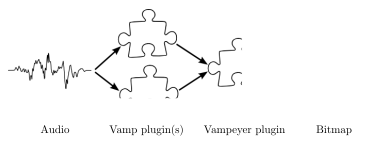
\includegraphics[width=0.8\textwidth]{figs/vampeyer.png}
  \caption{High-level system diagram of the Vampeyer visualization framework}
  \label{fig:vampeyer}
\end{figure}

The visualization plugin defines which Vamp plugin outputs it requires,
including the block/step size and parameters. At least one Vamp plugin is
required, but there is no restriction of the number of different Vamp plugins
that can be used.

Both frameworks are written in C++ which allows for a fast processing time.
This is important for situations where audio has to be processed on-the-fly,
such as for exploring an archive without having to pre-process everything in
it.  The plugins are compiled into shared libraries, so they can easily be
distributed without users having to recompile locally and integrated into
third-party software.

\subsection{Implementation}
A C++ header file was created which implements the design.  Five data
structures are also defined which define how data should be sent and returned
from the functions.

{\singlespacing
\begin{itemize}
  \item \texttt{VampParameter} is a name/value pair used to store a parameter
  \item \texttt{VampParameterList} is a vector of \texttt{VampParameter}s
  \item \texttt{VampPlugin} stores the name of a Vamp plugin along with a\\
    \texttt{VampParameterList} and the preferred block and step sizes
  \item \texttt{VampOutput} stores a \texttt{VampPlugin} and output name
  \item \texttt{VampOutputList} is a vector of \texttt{VampOutput}s
\end{itemize}
}

Two primary functions are used to define the input audio features and their
conversion to a bitmap.

\begin{itemize}
  \item \texttt{getVampPlugins} returns a \texttt{VampOutputList} variable
    that contains a list of Vamp plugin outputs which must be provided as
    input
  \item \texttt{ARGB} takes the Vamp plugin output data as a
    \texttt{Vamp::FeatureSet} variable, the sample rate of the audio and the
    desired width and height. It returns a bitmap image formatted in 32-bit
    ARGB format (alpha, red, green, blue).
\end{itemize}

A number of example plugins were written to demonstrate the capabilities of
this approach, and to act as useful pieces of software in their own right.
These include a standard waveform, waveform colourised by low energy ratio (see
Section~\ref{sec:studywaveform}), waveform colourised by spectral centroid
(identical to Freesound) and an MFCC grid visualization with waveform overlay.

The plugins need to be run by a host program which reads the audio data,
processes it using the Vamp plugins, sends their output to the visualization
plugin and then writes the image data. Such a program was written as a
command-line tool that can either display the image in a window or write it to
disk as a PNG-encoded file. This makes it useful for both prototyping and for
back-end processing on a server, for example.

\section{Browser-based audio interface}\label{sec:iface}
An audio interface was developed for use in evaluating a number of different
audio visualizations (see Section~\ref{sec:study}). In order to maximise the
number of people who could participate in the experiment, it was designed to be
accessible online and run in a web browser.

The latest web standards (such as HTML5) were exploited in order to ensure a
smooth and consistent user experience. This meant that some people running
older browsers were unable to take part, but the standards are mature enough
that the vast majority of browsers are compatible.

\subsection{Design}\label{sec:interfacedesign}
The screenshot of the  final design of the interface is shown in
Figure~\ref{fig:interface}, which includes of one the training pop-ups.

\begin{figure}[ht]
  \centering
  \includegraphics[width=\textwidth]{figs/interface.png}
  \caption{Experimental test interface with training pop-up}
  \label{fig:interface}
\end{figure}

\paragraph{Motivation}
The goal for the design was to include all the essential features required to
complete the task of finding and selecting a segment of audio (see
Section~\ref{sec:studytask}) in a way that can easily be picked up by novice
participants. Only the essential features were considered in order to make it
simple and to avoid distraction.

\paragraph{Displays}
Two displays were used -- one to show an overview of the entire recording, and
another showing an adjustable zoom display. It would be possible to complete
the task using only an adjustable zoom display, but it would be very difficult
to keep track of the position in the recording.

The zoom display was placed above the overview display and set to be slightly
larger than the overview in order to emphasise that the display is a
magnification. The two displays were linked using two curvy lines (splines)
which show the position of the zoom display limits in the overview display.

The current position of the audio playback was signified by adding a `cursor'
using a line on each display. The cursor can be moved by clicking or dragging
on either of the displays using the mouse.

Selected areas of audio are highlighted using a semi-transparent overlay which
appears on both displays.  A time `ruler' was also overlaid on both displays to
give users an objective scale and a sense of the relative scale of the
displays.

\paragraph{Zoom control}
The level of zoom was controlled using two buttons at the bottom -- one to zoom
in and another to zoom out. In an early prototype, users could press these
buttons as many times as they wished, but this caused confusion when maximum
zoom was reached and the button stopped doing anything. Following feedback,
this was rectified by disabling and greying out the buttons when at max/min
zoom.

\paragraph{Selection}
Two methods of selecting content were implemented -- one using buttons and
another using a slider. The buttons were used to set either the in or out point
of the selection to the current position of the cursor. The buttons could be
used while the audio is playing, allowing users to press a button as they hear
their preferred start/end point. As the cursor can be moved on the zoomable
display, the buttons can be used to set the selection precisely.

The slider acts both as a display of where the selection is and as a method of
setting or adjusting it. The slider was located just under the overview display
and has `handles' on each side which can be dragged to adjust the start and end
of the selection. After receiving feedback on a prototype, the slider was
configured to update the highlight in the displays as it is dragged, making
fine adjustments easier to see.

\paragraph{Training}
Although the interface is relatively basic as far as digital audio workstations
are concerned, a system was developed to train users in the features and
operation of the interface. This was done using a `pop-up tour', which is
a technique often found on web pages. It involves a series of dialog boxes
which point out different parts of the interface with some text explaining what
they do. You can see an example in Figure~\ref{fig:interface}.

\subsection{Implementation}

\paragraph{Front-end}
A feature-heavy web page, such one that includes an audio/visual interface, can
be slow to load and unresponsive. To avoid this, the interface was set up as a
`single-page application' which loads the content of each page dynamically
without having to reload the interface and the large Javascript libraries that
it's built on.

Angular.JS\footnote{\url{https://angularjs.org}} is a Javascript web
application framework which aids development of dynamic web pages. A
single-page application was implemented using its `route' and `view' features.
Its other features were used to send responses to the database and update the
cursor/selection on the visualization, amongst other things.

Bootstrap\footnote{\url{http://getbootstrap.com/}} was used to style the page
and the components in it. The popularity of Bootstrap means that this style is
familiar and comfortable to most web users. Bootstrap
Tour\footnote{\url{http://bootstraptour.com/}} is a Javascript library for
running `pop-up tours' on websites. This was used to implement the training
interface, as discussed in Section~\ref{sec:interfacedesign}.

\paragraph{Back-end}
A web server and database were used to serve the web pages and experimental
data, and to store the results. Node.js\footnote{\url{http://nodejs.org/}} was
used to implement and expose an API for interacting with the front-end and
CouchDB\footnote{\url{http://couchdb.apache.org/}} was used as the database.

The sequence for each experiment (described in Section~\ref{sec:studysequence})
needed to be assigned to participants evenly, so that each sequence is
completed exactly once before a second participant is assigned to it. This was
done by taking the sequences that had been completed the least number of times,
then choosing the sequence that had been assigned the longest time ago (or not
at all). This approach minimised the chance of more than one participant using
the same sequence. 

\paragraph{Audio playback}
Different browsers support a variety of different audio codecs and have
different capabilities in terms of playback methods. In order to maximise
compatibility, SoundJS\footnote{\url{http://www.createjs.com/\#!/SoundJS}} was
used to play the audio content.

The audio content was data compressed using a lossy codec to reduce the size
(and therefore loading time) of each web page. Ogg Vorbis was used as the
primary codec, with a quality setting of 2 (approx. 80kbps VBR). For browsers
that didn't support Ogg Vorbis, AAC was used with a variable bitrate of 96kbps.
The use of lossy codecs introduces some audible artefacts. However this is not
part of the experiment and it impacts every audio clip, so is not expected to
bias the results. 

\paragraph{Visualization}
The duration of each of the audio clips used in the experiment is about 5
minutes, and the interface display allows for four levels of zoom. This
produces up to $\sim$2MB of image data which, if loaded at the beginning, would
negatively impact on the loading time of the web page. To fix this, a tiling
system was used where each image was cut into tiles 240 pixels wide. The
displays then dynamically loaded the tiles as and when they were needed.

To ensure maximum browser compatibility and to simplify the implementation,
KineticJS\footnote{\url{http://kineticjs.com/}} was used to render the images,
ruler and cursor.



\chapter{Navigation of timed transcripts}



\begin{appendices}
  \section{Service remits and conditions}\label{app:remit}

\paragraph{Radio 1}
``to entertain and engage a broad range of young listeners with a distinctive
mix of contemporary music and speech''

\begin{itemize}
  \item $\geq$ 60 hours specialist music each week
  \item $\geq$ 25 major live events and festivals each year
  \item $\geq$ 250 new sessions each year
  \item $\geq$ 1 hour of news each weekday
  \item $\geq$ 40 new documentaries each year
\end{itemize} 

\paragraph{Radio 1Xtra}
``to play the best in contemporary black music with a strong emphasis on live
music and supporting new UK artists''

\begin{itemize}
  \item $\geq$ 20\% of output is speech-based
  \item $\geq$ 1 hour of news each weekday
\end{itemize}

\paragraph{Radio 2}
``to be a distinctive mixed music and speech service, targeted at a broad
audience, appealing to all age groups over 35''

\begin{itemize}
  \item $\geq$ 260 hours of live music each year
  \item $\geq$ 16 hours of news and current affairs each week
  \item $\geq$ 130 hours of documentaries each year
\end{itemize}

\paragraph{Radio 3}
``to offer a mix of music and cultural programming in order to engage and
entertain its audience''

\begin{itemize}
  \item $\geq$ 40\% of music output is live or specially recorded
  \item $\geq$ 400 live or specially recorded performances each year
  \item $\geq$ 25 new drama productions each year
  \item $\geq$ 30 new documentaries on arts and cultural topics
\end{itemize}

\paragraph{Radio 4}
``to be a mixed speech service, offering in-depth news and current affairs and
a wide range of other speech output including drama, readings, comedy, factual
and magazine programmes''

\begin{itemize}
  \item $\geq$ 2,500 hours of news and current affairs each year
  \item $\geq$ 600 hours of original drama each year
  \item $\geq$ 180 hours of original comedy each year
  \item $\geq$ 350 hours of original documentaries each year
\end{itemize}

\paragraph{Radio 4 Extra}
``to provide speech-based entertainment. Its schedule should include comedy,
drama, stories, features, readings and programmes that appeal to children''

\begin{itemize}
  \item $\geq$ 55 hours of comedy each week
  \item $\geq$ 55 hours of drama each week
  \item $\geq$ 350 hours of childrens programming each year
\end{itemize}

\paragraph{Radio 5 Live}
``to provide live news and sports coverage''

\begin{itemize}
  \item 75\% of output is news and current affairs
\end{itemize}

\paragraph{Radio 5 Live Sports Extra}
``to bring a greater choice of live action to sports fans by offering a
part-time extension of BBC Radio 5 live''

\paragraph{6 Music}
``to entertain lovers of popular music with a service that celebrates the
alternative spirit in popular music from the 1960s to the present day''

\begin{itemize}
  \item $\geq$ 400 hours of archive concert performances each year
  \item $\geq$ 15\% of music is concert tracks and sessions each year
  \item $\geq$ 300 new sessions each year
  \item $\geq$ 10 hours of speech-based features each week
  \item $\geq$ 6 hours of news each week
\end{itemize}

\paragraph{Asian Network}
``to provide speech and music output appealing to British Asians, with a strong
focus on news and current affairs''

\begin{itemize}
  \item Content is approximately 50\% music and 50\% speech during the daytime
  \item $\geq$ 10\% of music is South Asian
  \item $\geq$ 20 hours of language programming each week, including a mixture
    of Hindi/Urdu, English and other regional languages
\end{itemize}


  \chapter{Startrack interface description}\label{app:startrack}
This section provides details of the most common operations and how they are
achieved in StarTrack.

\begin{figure}[ht]
\centering
\includegraphics[width=0.8\textwidth]{figs/startrack.png}
\caption{The user interface for StarTrack.}
\label{fig:startrack}
\end{figure}

\paragraph{Modes}
There are three modes in which the StarTrack interface can operate. The default
-- `\textbf{edit mode}' -- is where audio clips can be cut and trimmed,
`\textbf{arrange mode}' is targeted towards moving clips around and
`\textbf{level mode}' is for editing level automation

The primary difference between the modes is the behaviour of the mouse. In
edit mode, clicking the left button sets the position of the cursor, the right
button allows clips to be moved, and dragging with the left button makes a
selection of audio. In arrange mode, the left button selects clips, dragging
moves them around and the middle button sets the position of the cursor. In
level mode, the mouse can be used to move, create and delete nodes in the level
automation.
% what does the right button do?

\paragraph{Playback}
The interface contains five play modes, which were chosen to cater for the most
common editing tasks. They are listed below with their keyboard shortcuts. The
default for $x$ is 2.

\begin{itemize}
  \item \texttt{[space]} Normal playback
  \item \texttt{[B]} Play $x$ seconds from cursor position - used to check
    intro before topping clip. \texttt{[Backspace]} operates in a similar way,
    but with a 5 second lead-up.
  \item \texttt{[V]} Play $x$ seconds up to cursor position - used to check
    outro before tailing clip
  \item \texttt{[N]} Play first and last $x$ seconds of selection - used to
    check selection before clipping
  \item \texttt{[M]} Play $x$ seconds before and $x$ seconds after selection -
    used to check selection before deleting\footnote{This method does not
      perform a crossfade so is not an accurate representation of how an edit
      would sound}
\end{itemize}

The speed of playback can be controlled using the \texttt{[$\uparrow$]} and
\texttt{[$\downarrow$]} buttons, which increases/decreases the rate at which
the audio samples are played (giving a `chipmunk' effect on speech). Pressing
\texttt{[$\downarrow$]} enough times reverses the direction of playback.

\paragraph{View}
The view can be manipluated in a number of ways. The height of the selected
track (vertical zoom) can be controlled with \texttt{[Page Up]}/\texttt{[Page
  Down]}, or by using the mouse to drag the boundaries between tracks. The time
span (horizontal zoom) can be controlled with \texttt{[+]}/\texttt{[-]}, or by
holding \texttt{[Ctrl]} and using the mouse scroll wheel. When some audio is
selected, pressing \texttt{[=]} fits the selection to the window (zoom to
selection).

Each clip has an associated colour and name, which are displayed using the
waveform and a label underneath. These can be changed by right-clicking the
clip and using the context menu.

Markers can be set using the \texttt{[\#]} key and they appear as a triangle at
the top of the track. Each marker has an associated colour and label, although
the label isn't visible. They can be edited by right-clicking on the marker.
Markers are affixed to the audio data, so they remain in place when clips are
copied or moved.

\paragraph{Navigation}
In addition to using the mouse to navigate (as described in the `modes'
section), navigation and selection is aided through the use of a number of
shortcuts:
\begin{itemize}
  \item \texttt{[$\leftarrow$]}/\texttt{[$\rightarrow$]} Move to the
    previous/next edit point or marker. Use with \texttt{[$\Uparrow$]} to move
    to beginning/end of selection.
  \item \texttt{[Home]/[End]} Select to start/end of clip. Use with
    \texttt{[Ctrl]} to move the cursor
  \item \texttt{[7]/[8]} Nudge/nibble the start of the selection left/right
  \item \texttt{[9]/[0]} Nudge/nibble the end of the selection left/right
  \item \texttt{[ / ]} Set in/out markers for selection while playing
\end{itemize}

\paragraph{Editing}

\verb$[\]$ splits a clip into two at the point of the cursor. A solid line
shows that the clip is not connected, and the two parts can be moved freely.

\texttt{[Delete]} removes a selection of audio from a clip and joins the two
remaining parts of the clip together with a crossfade. The edit is shown as a
dotted line with an empty triangle at the top, indicating that the two
remaining parts are connected and move together. The user can undo the edit at
a later stage by right-clicking the triangle and selecting `undo edit'.

\texttt{[w]} removes the selected audio, but separates the remaining two parts
into individual clips and leaves a gap in the middle.

Fade in/out operations must be done using the mouse. There is a triangle in the
top left/right corner of each clip which, when dragged, applies a fade in/out.
It can also be done by making a selection and using the context menu, which has
three curve options.

When clips overlap on a track, their output is played simultaneously. Any
crossfading between the two must be done manually by using level automation.

\paragraph{Levels}
By default, each clip displays a solid horizontal black line which represents a
0dB gain for that clip. It can be moved up and down with the mouse in edit
mode. Holding \texttt{[Ctrl]} changes the level only in the selected region and
holding \texttt{[$\Uparrow$]} affects all of the clips in that track.

Switching to level mode allows finer control using level automation. Nodes can
be created by dragging the first/last node in a clip, or holding
\texttt{[Ctrl]} while clicking on the black line. Nodes can be deleted by
holding \texttt{[Ctrl]} and clicking on an existing node.

\paragraph{Takeboard and clipboard}
The `takeboard' is a list displayed on the right of the interface which
contains a list of all raw audio recordings that are available. They can be
dragged and dropped onto a track.

The `clipboard' contains a list of clips. In this context, a `clip' is a copy
of an edit, which can be made by highlighting part of a track and pressing
\texttt{[C]}. The clip will include any level automation and can include parts
of multiple audio files and silences. In that respect, it can be considered to
be a mini EDL. Deleting a clip does not destroy any raw audio data.

The list of clips can be reordered, and by selecting multiple clips from the
list and dragging them onto a track, they will be inserted one after the other.
This functionality is useful for putting together a rough edit.  Pressing
\texttt{[P]} will preview the selected clip in a small preview window. The
preview only contains play, stop and scroll functionality, but audio can be
selected and dragged onto a track. Clips can be `bounced down' to an audio file
using the context menu.

\paragraph{Slips and chains}
When audio clips (or parts of clips) are removed\slash inserted\slash moved,
the clips to the right of the edit on that track are automatically moved to
fill/accomodate the edit. When multiple tracks are used, this can cause tracks
to fall out-of-sync with each other, but this can be fixed by using either
chaining or slipping.

Chaining is where multiple tracks are grouped together so that when audio is
removed\slash inserted\slash moved, all of the clips on the chained tracks move
together.  When audio is selected on a chained track, it is selected across all
of the chained tracks.

Slipping is similar to chaining but affects all tracks, not just those chained
together. StarTrack provides the option of `right slip', where clips on every
track to the right of the edit move together, or `left slip' where the clips to
the left of the edit move together. Both can be used at the same time, which
gives the effect of chaining all tracks.

Tracks can also be locked so that they are unaffected by actions in other
tracks. This is useful for content such as background music, which doesn't need
to be in sync.

\paragraph{Signal processing}
StarTrack includes support for VST audio effect plugins. A number of
VCS-branded plugins are supplied as standard, including ones for dynamics,
parametric EQ, graphic EQ and mixing. A simulated PPM meter is also available
for checking levels. However, the VST support in StarTrack is currently limited
to VST v2.0, can only support stereo signals and doesn't support channel
mapping. Parametric EQ can also be applied to clips individually through a menu
option.

\paragraph{Saving and bouncing down}
Projects can be saved either `without audio', where the audio data remains
stored in the dira! system, or `with audio', where the audio is copied onto the
local machine. BBC best practise stipulates that the audio should be stored on
dira! whenever possible in order to avoid data loss and to make the files
available to other staff members.

StarTrack performs a local background autosave every two minutes where projects
can be restored through a menu option. When a project is `bounced down' to an
audio file, only the tracks which are visible in the interface are included in
the mix. This can be useful for easily excluding tracks, but is usual behaviour
for a DAW, so could catch people out.

  \chapter{Consent form}\label{app:consent}
You are invited to participate in this research study examining the performance
of audio waveforms. The purpose of this page is to provide you with information
required for you to make an informed decision regarding participation in this
research.

\paragraph{What you will be asked to do}
If you agree to participate in this experiment, you will be presented with a
sequence of nine audio recordings and asked to select the music within each
recording. The audio waveform will change throughout the experiment and you
will be asked to rate the performance of each. At the end, you will be asked to
compare them.

It is anticipated that the entire experiment will take between 10 and 15
minutes. You can complete the experiment at a time and location that is
convenient to you. You can also save your progress by creating a bookmark and
completing the experiment at a later date.

\paragraph{Voluntariness}
Participation in this study is voluntary. You may refuse to participate, refuse
to answer any questions or withdraw from the study at any time without any
consequences to you. If you wish to withdraw from the study after having
completed the task, you can do so by sending the ID code below, along with the
request to have your responses removed, to the researcher within 24 hours of
completion.

Your ID code is xxxxxx.

\paragraph{What information will be collected}
{\singlespacing
\begin{itemize}
\item Your browser and OS details
\item Your demographic information
\item Your actions during the tasks
\item Your ratings of the tasks and waveforms
\item The date/time you completed the tasks
\end{itemize}
}

\paragraph{Confidentiality}
No personally identifiable information will be collected during the experiment.
The data and results of this study may be published, but in no way that will
allow you to be identified.

\paragraph{Conditions}
To participate in this study your vision and hearing must be unimpaired and you
have to be at least 18 years old. There are no known or anticipated risks or
discomforts associated with participating in this study. You will not be
monetarily compensated for your participation in this research.

\paragraph{Further information}
If you require any further information regarding this research project or your
participation in the study you may contact Chris Baume
(\url{chris.baume@bbc.co.uk}).  The results of the experiment will be made
available on the following website:
\url{http://www.bbc.co.uk/rd/projects/audio-visualization}

\mbox{}\\
\noindent
\textbf{"I, the participant, have read the above information and wish to
  participate in this study"} [Agree/Disagree]

  \chapter{BBC radio production workflow}\label{sec:production}
BBC radio is a huge operation with 59 radio stations spread across the UK
covering every type of programme and music genre. Successfully documenting the
entire system would be difficult if not impossible as different groups and
departments have wildly varying ways of accomplishing the same task.

This section aims to provide a high-level overview of the most common
processes, systems, interfaces and language used in BBC radio production. It
will provide some context to the real-life environment for which the work in
this project will eventually feed into, and may help guide the direction of the
research.

\section{Roles}\label{sec:roles}

\paragraph{Producer}
Most radio programmes have one producer who `owns' that programme.  In many
cases, about 80\% of the time spent creating the production is done so by the
producer. In addition to controlling the editorial content, they usually make
the audio recordings and do most of the audio editing. Producers usually only
receive half a day of official training with the rest learnt `on-the-job'.

\paragraph{Presenter/Reporter}
The presenter is the voice of the programme. They provide the links and conduct
interviews with the contributors. In some cases, they work closely with the
producer on the editorial content.

\paragraph{Journalist}
This role is more common in the News division, and the role is usually a
combination of producer and presenter. The emphasis for journalists is on
newsgathering.

\paragraph{Editor}
Editors are senior producers who have a significant amount of experience. They
provide editorial guidance to producers and are often involved with the
programme compliance.

\paragraph{Studio Manager}
The studio manager is responsible for the audio output of the programme. Often
they only get involved at the very end of a production to clean up any rough
edits and apply noise reduction/EQ. In live productions, they operate the
mixing desk and set up remote contributions. In News, senior studio managers
are called Studio Directors.

%\subsection{Commissioner}
%When a producer has an idea for a programme, they pitch that idea to a
%commissioner who then decides whether it gets made.

%\subsection{Broadcast Assistant}

\paragraph{Media Manager}
Ingests video and audio content for News by setting up ISDN links and BNCS
routing, creating clips from incoming feeds and attaching basic metadata.

\subsection{Political structure}\label{sec:organisation}
BBC radio output is produced across three top-level divisions - Radio (formerly
called Audio \& Music), News and North. The structure is listed below.

\begin{itemize}
  \item Radio
  \begin{itemize}
    \item Radio 1, 1Xtra
    \item Radio 2, 6 Music, Asian Network
    \item Radio 3
    \item Radio 4, Radio 4 Extra
    \item Production
    \begin{itemize}
      \item Factual
      \item Arts, Documentaries and Drama
    \end{itemize}
    \item Live Music, Events and Popular Music
  \end{itemize}
  \item News
\end{itemize}

\subsection{Services}
The BBC broadcasts a diverse range of speech and music content across genres
including news, drama, comedy, live events, magazine shows, documentaries,
cultural programming and childrens. Quantifying the proportion of these types
of content is difficult as there is little metadata or publications that go
into that level of detail. However, the BBC Trust publishes an annual radio
service
licence\footnote{\url{http://www.bbc.co.uk/bbctrust/our_work/services/radio/service_licences.html}}
which sets aims and objectives for the content of each network. The remits also
include specific conditions which can significantly affect the audio content
(e.g. ratio of music/speech). Using these, it is possible to gauge the
character of each radio network and at least a minimum level of different
content types. The remits and conditions are listed in
Appendix~\ref{app:remit}.

Six of the networks are characterised as a mix of music and speech, with the
other four being purely speech-based. This demonstrates that much more
speech-based audio content is broadcast than music. Of the speech content, much
is likely to be news and current affairs as all of the networks include it to a
greater or lesser extent, and two networks are dedicated to it. With music,
there are a number of conditions that encourage or demand live music and
performances, although the majority of music output will be recordings.

\section{Technology}\label{sec:workflow}
The audio workflow at the BBC is vast and complicated. Despite attempts to
harmonise production tools, the wide variety of requirements from production
staff around the BBC means that no one tool can cater for everyone. For
example, some content is turned around in a few minutes whilst other content
could be worked on for a month. However, even though there are plenty of
options available, on a day-to-day basis most producers get by using only the
dira! system.

It would be impractical to capture every single component that audio content
touches at the BBC, so this report will only attempt to detail the most common
systems.  Figure~\ref{fig:workflow} shows a typical audio data flow for radio
production in the BBC.

\begin{figure}[ht]
\centering
\includegraphics[width=\textwidth]{figs/workflow.pdf}
\caption{Typical flow diagram for audio data in BBC Radio.}
\label{fig:workflow}
\end{figure}

\section{Ingest}\label{sec:ingest}
The chosen method of capturing audio content is highly dependent on the type of
programme that is being made. For instance, phone-in shows will combine live
studio recordings with telephone links, and news reports will primarily use
portable recorders. 

\paragraph{Studio recordings}
An obvious but important source of audio content is studio recordings. A
typical set-up consists of an acoustically isolated studio containing a number
of microphones. The studio is connected via triple-glazed windows to one or two
acoustically treated cubicles housing a mixing desk and monitors. The presenter
and guests sit in the studio and the studio manager and producers sit in the
cubicle.

\paragraph{Telephony}
POTS\footnote{Plain old telephone service -- standard phone line} is still used
heavily as it is often the only practical method of setting up remote
contributions on short notice or to members of the public (such as for Radio
4's `Any Answers?' programme).  Where a contribution is planned in advance, an
ISDN\footnote{Integrated Services for Digital Network -- 128kbps digital phone
  connection} link can be set up to a local studio, or to a location equipped
with a ISDN codec box (such as stadiums). This gives a much higher sound
quality but can be expensive if a connection is not already in place.
Increasingly, Internet protocol (IP) links are being used for remote audio
contributions.  Skype is readily used in place of POTS due to its higher sound
quality, and hardware from Comrex (such as its ACCESS and BRIC products) is
being increasingly used to provide high quality contribution links.

\paragraph{Portable recorders}
Recordings made on location are most often made with a microphone and portable
recorder\footnote{Sometimes referred to as a `Nagra' -- a popular brand of
recorder}. The audio, which is stored on Compact Flash or SD cards, is then
either physically taken back to the office or transferred over the Internet
through the use of an FTP server or a browser-based online service provided by
Arbor Media, which automatically copies the recordings into dira!.

\paragraph{Simulrec}
This is a common technique which is used to increase the sound quality of
conversations between a presenter in the studio and a contributor on the
telephone. The interview is conducted over the phone, but each side of the
conversation is also recorded locally using broadcast quality microphones. In
the studio, the recording is made using an audio editor. The contributor is
recorded with a portable recorder and the recording is sent over the Internet
to the studio, where it is imported and lined-up in the audio editor. The
result makes it sound as if the conversation happened in the same room.

\paragraph{Archive} Many programmes require the use of previously-broadcast
material which is stored in one of many archives.

\paragraph{AutoROT} Automatic Record of Transmission (see
Figure~\ref{fig:autorot}) is a popular system that records all network radio
output, plus a number of other streams including the feed from the House of
Commons.  Some of its content stretches back as far as November 2006.  It is
accessed using an online GUI which allows users to audition, clip and download
content.  AutoROT contains a mixture of uncompressed .wav recordings, which are
suitable for re-use, and data-compressed recordings, which are only suitable
for research/browsing.

\paragraph{Jupiter} BBC News store all of their video content in the Jupiter
system, which can be accessed through an online web interface called Davina.
Although not designed specifically for audio content, Jupiter is often used to
take audio data from video recordings.  It is possible to edit audio using a
video editor with Jupiter, but often it is easier to copy the audio content to
dira! and use a program like StarTrack.

\begin{figure}[p]
\centering
\includegraphics[width=0.8\textwidth]{figs/autorot.png}
\caption{User interface for BBC AutoROT.}
\label{fig:autorot}
\end{figure}

\begin{figure}[p]
\centering
\includegraphics[width=0.8\textwidth]{figs/snippets.png}
\caption{User interface for BBC Snippets for Radio.}
\label{fig:snippets}
\end{figure}

\paragraph{I\&A catalogue}
The BBC's physical archive is managed by the Information and Archives
department, who are primarily based in Perivale. Material can be either be
searched for using the legacy INFAX system or through the new Fabric platform,
both of which are browser-based. Material is found using text-based search
and is then ordered via a phone call. The recording is then either digitised
and deposited in a shared network drive, or the physical media is sent to the
producer via internal mail.

\paragraph{Radio Digital Archive}
The Radio Digital Archive (RDA), and its predecessor the Radio Interim Archive
(RIA), capture all network radio output in uncompressed PCM format. The RIA
started in August 2008 with the RDA taking over in March 2013. They contain
recordings of transmission, pre-recorded items, extended interviews and music
sessions. The RIA stores content as .wav files segmented into 30 or 60-minute
chunks. The RDA uses information from Coyopa (see Section~\ref{sec:coyopa})  to
segment the audio at programme boundaries and to include programme metadata.

\paragraph{Redux}
BBC Redux is an experimental system run by BBC R\&D which records all BBC
television and radio output. It has been running since July 2007. It differs
from other ROT systems in that it records content off-air (via FreeSat). As the
content is data-compressed, it is not fit for broadcast and only used for
programme-making when other archives have been exhausted.

\paragraph{Snippets}
In 2012, a new user interface was developed to allow advanced search and
navigation of Redux. The project, named Snippets, adds features such as the
ability to search the text of television subtitles, audition, clip (`snip') and
download content in-browser and search by cast/crew. The recently introduced
`Snippets for Radio' allows users to navigate radio content with a waveform
display and keyboard shortcuts (see Figure~\ref{fig:snippets}). The code which
powers Snippets for Radio has been open-sourced\footnote{See
  \url{http://waveform.prototyping.bbc.co.uk}}.

\section{Storage}

\paragraph{dira! Highlander}
The dira! radio production system is central to the BBC's operation. Almost all
non-live audio content is stored, edited and played out using the system. Dira!
was originally manufactured by a company called \textbf{VCS}, which was then
bought in 2012 by SCISYS. However, within the BBC almost everybody refers to
the dira! system as VCS because of the branding on the software and equipment.

The Highlander program is the user interface for accessing the dira! database
(see Figure~\ref{fig:highlander}). The entire dira! system spans a number of
servers, but Highlander can access only one at a time. Each server consists of
a folder structure where each folder contains a number of `\textbf{stores}'.
The stores contain a `\textbf{take list}' consisting of audio recordings and
StarTrack EDLs\footnote{Edit Decision Lists}.

\begin{figure}[p]
\centering
\includegraphics[width=0.9\textwidth]{figs/highlander-interface.png}
\caption{User interface for dira! Highlander.}
\label{fig:highlander}
\end{figure}

Although the stores are technically identical, they are manually arranged to be
used for different purposes, such as:
\begin{itemize}
  \item \textbf{Programme stores}, for regular programmes (such as Woman's
    Hour)
  \item \textbf{Generic stores}, for other programmes in a given network (such
    as Radio 2)
  \item \textbf{Music stores}, for storing music tracks
  \item \textbf{Recording stores}, for raw studio recordings, recordings of
    transmission and presenter links
\end{itemize}

Each store has an individual capacity and expiration time, after which items
are moved to a `\textbf{recycle bin}'. The recycle bin has a 72 hour expiry
time, after which items are unrecoverable. The capacity/expiration parameters
vary for each store, depending on its use. For instance, stores for regular
programmes expire after 30 days, whilst the music stores never expire.

\begin{figure}[p]
\centering
\includegraphics[width=0.9\textwidth]{figs/audition-interface.png}
\caption{User interface for dira! Highlander audition window.}
\label{fig:highlanderaudition}
\end{figure}

Each audio item has a yellow speaker icon which brings up an audition window
(see Figure~\ref{fig:highlanderaudition}) for playing and navigating the clip.
No editing facilities are provided, but there is a button for sending the audio
clip to the StarTrack editor.

Edit decision lists (EDLs) have a folder icon with the letter `A' associated
with them. When selected, they can be opened with the `send to editor' button.

\begin{figure}[p]
\centering
\includegraphics[width=0.8\textwidth]{figs/take-data-card.png}
\caption{Take data card window in dira! Highlander.}
\label{fig:takedatacard}
\end{figure}

Double-clicking on an item opens the `\textbf{take data card}' or `TDC' (see
Figure~\ref{fig:takedatacard}) which is used to read and enter metadata. Some
fields are compulsory and are highlighted in red, and the others are filled in
subject local conventions. There are different types of TDCs for different
types of content. Those which store audio content are called `\textbf{DIGA}s'. 
% explain what EXTA is

\begin{figure}[p]
\centering
\includegraphics[width=0.8\textwidth]{figs/highlander-filter.png}
\caption{Take list filter window in dira! Highlander.}
\label{fig:highlanderfilter}
\end{figure}

Items can be found by browsing the take list, which can be sorted by title,
duration, time of creation/last modification and username of creator/last
modifier amongst others. The items in the take list can be filtered by text
search, including wildcards (see Figure~\ref{fig:highlanderfilter}), or the
whole server can be searched at once with the results appearing in a separate
window.

\begin{figure}[p]
\centering
\includegraphics[width=0.8\textwidth]{figs/ats-recorder.png}
\caption{The user interface for ATS recorder in dira! Highlander.}
\label{fig:atsrecorder}
\end{figure}

Audio can be ingested into Highlander by importing a file, making a live
recording or ripping a CD. Imported files are normalised before being uploaded
to the database. The live recordings are made using the `\textbf{ATS recorder}'
program. The interface (see Figure~\ref{fig:atsrecorder}) includes a VU meter,
simple faders, and a button for creating markers. CDs can be extracted using
the CDExtract program, which automatically grabs the CD metadata from an
external database.

\paragraph{Shared network drive}
Audio content is often stored in Windows network fileshares which are mounted
as part of the standard IT infrastructure. Until recently, audio content was
stored in a share mounted as `M:' and known as the `M drive'. This has recently
been replaced with a share mounted as `S:'. The `S drive' is is a disaster
recovery server whose data is split across three sites. Broadcast critical
audio content stored in dira! is automatically copied to S: so that it can be
used if the dira! system fails. However it is also used as a conventional
network drive to store and share content.

\paragraph{Portable hard drives}
Portable USB and Firewire hard drives are popular for transferring and storing
files, despite the risk of data loss. They are often referred to as `Lacie
drives' due to the prevalence of bright orange LaCie-branded drives in the BBC.
Their use is most common when handling large data files which the network can
struggle with, or for storing data when network access is unavailable, such as
on location.

\section{Editing}

\begin{figure}[p]
\centering
\includegraphics[width=0.8\textwidth]{figs/startrack.png}
\caption{The user interface for StarTrack.}
\label{fig:startrack}
\end{figure}

\paragraph{StarTrack}\label{sec:startrack}
This is widely used throughout the BBC for editing audio content. It is a
multi-track digital audio workstation which provides all the basic editing
facilities a producer would normally require. It is popular due to its tight
integration with dira! and its simple interface, relative to other DAWs (see
Figure~\ref{fig:startrack}).  StarTrack is limited to 16 tracks and is only
able to handle mono and stereo content.

A detailed description of common operations and how they are achieved can be
found in Appendix~\ref{app:startrack}.

\begin{figure}[p]
\centering
\includegraphics[width=0.8\textwidth]{figs/orion.png}
\caption{The user interface for Orion.}
\label{fig:orion}
\end{figure}

\paragraph{Orion}
This is a single track editor designed for very quick and basic audio edits,
such as level adjustment and top/tailing. It is commonly used within News for
its ability to create clips from incoming live audio feeds as they're being
recorded. Orion is very similar to StarTrack in that it has identical keyboard
shortcuts and includes most of the same features, apart from multiple tracks,
level automation and signal processing, for example.

Notably, when the audio is replayed at greater than normal speed, instead of
playing the samples faster like StarTrack does, Orion skips short segments.
This gives the audio a `choppy' effect, rather than a `chipmunk' effect, but is
more intelligible for some.

\paragraph{SADiE}
This is an advanced digital audio workstation used for more complicated edits
such as for music recordings and documentaries. This is sometimes referred to
as `craft editing'. Certain areas of the BBC, like the Science unit and Radio
3, use SADiE routinely, but in most other areas its use is exceptional.

\begin{figure}[p]
\centering
\includegraphics[width=0.8\textwidth]{figs/sadie.png}
\caption{The user interface for SADiE 6.}
\label{fig:sadie}
\end{figure}

SADiE supports a number of extra features not found in StarTrack:
\begin{itemize}
  \item More than 16 tracks
  \item Multi-channel
  \item External audio interfaces
  \item Hardware controllers (e.g. jog wheel)
  \item Larger plugin selection (supports all VSTs)
  \item Channel mixing/routing
\end{itemize}

The interface for SADiE (see Figure~\ref{fig:sadie}) is more complicated, but
is highly customisable and uses a much better waveform renderer.

A plugin package from iZotope is included with SADiE, which included a
multiband compressor, reverb, delay, flanger etc. It also supports all versions
of VST plugins, allowing a much greater selection than StarTrack which only
supports VST v2.0.

\begin{figure}[p]
\centering
\includegraphics[width=0.8\textwidth]{figs/sadie-controller.jpg}
\caption{A SADiE hardware controller.}
\label{fig:sadie-controller}
\end{figure}

Most common tasks in SADiE can be achieved with its custom hardware controller
(see Figure~\ref{fig:sadie-controller}). These units are common throughout the
BBC and are widely used by those with lots of experience with SADiE. They are
popular because most editing tasks can be achieved more efficiently than with a
mouse and keyboard.

Projects can be converted between SADiE and StarTrack using one of two programs
-- Transporter and SSL Pro--Convert. Although they support basic edits, more
advanced features are not supported, so it is rare for SADiE projects to be
converted to StarTrack.

\paragraph{Audition}
Adobe Audition is used in a similarly way to SADiE, but its use is more popular
in News than Radio. This may be because historically, SADiE workstations could
not be used without dedicated hardware, making them impractical for use
off-site. Cool Edit Pro was used instead, which was then bought by Adobe and
turned into Audition.

\section{Metadata}
Metadata is information about data. In the case of radio, it is information
about the audio content. This can include anything from who made a programme to
where particular recordings were made. Collection and use of metadata has
received an increasing amount of attention since the late 1990s as its
importance is recognised. There are two main systems used to collect metadata
on radio productions.

\paragraph{Proteus}
Proteus is a database designed for storing a wide variety of information about
radio programmes. It has been developed by an in-house BBC Radio team since
2001. It can be accessed using a modern browser-based interface (see
Figure~\ref{fig:proteus}). Some of the information it can store includes:
\begin{itemize}
  \item Transmission schedule
  \item Running order
  \item Contributors
  \item Music reporting
  \item Compliance
  \item Descriptions (for iPlayer)
  \item Recordings
  \item Rights
\end{itemize}

\begin{figure}[p]
\centering
\includegraphics[width=\textwidth]{figs/proteus.png}
\caption{The user interface for Proteus, showing the running order of an
  episode of Woman's Hour.}
\label{fig:proteus}
\end{figure}

There is no requirement to use the system, so different networks and programmes
use the system to varying degrees depending on local convention. Proteus also
duplicates functionality that is found elsewhere, such as music reporting which
can be done in Highlander. 

Each person who uses Proteus does so with a personal account which gives them
different levels of permissions. The system also records the actions performed
by users, which provides version control and audit capabilities. This setup
means that it can be used to co-ordinate approvals for compliance and edit
public-facing information such as the descriptions which feed into iPlayer.

Radio 1, 1 Xtra and 5 Live make minimal use of Proteus as they uses dira! for
music reporting and PowerGold for music rotation. Radio 2 puts presenter
information in, but little else. Radio 3 enters the production team information
and all of the music that is played as its music rotation software relies on
Proteus. Radio 4 uses Proteus more than any major network, particularly shows
such as `You and Yours' and `Woman's Hour', which make full use of the system's
functionality. 

Proteus can be accessed using an API.

\paragraph{Scheduler}
Scheduler is part of the dira! system and allows producers to create a schedule
of programmes and attach metadata to them. Each `programme slot' stores a list
of `elements' which can include text and audio items. The timing of each
element is managed to help the producer plan the programme length. A music
programme, for example, may consist of a track list of dira! audio items (from
a music store) with textual notes between tracks which the presented can use
either as a script or prompts for items to discuss. 

\paragraph{PIPs}\label{sec:pips}
Program Information Platform (known as PIPs) is a database containing
public-facing metadata on BBC TV and radio programmes. It was originally set up
to supply external listings such as Radio Times, but has expanded to feed
the BBC `/programmes' website and iPlayer. Each episode, series and brand has a
unique ID called a programme ID (or \textbf{PID}) made up of eight letters and
numbers (e.g. The Now Show is \texttt{b006qgt7}).

The information stored in PIPs includes:
\begin{itemize}
  \item Schedule
  \item Descriptions
  \item Images
  \item Segments/tracklists
  \item Links
  \item Keywords
\end{itemize}

Much of the data in PIPs is collected automatically from other systems. For
instance, the schedule, title and descriptions are pulled from Proteus, while
tracklistings are pulled from dira!. Further information can be added/edited
using a system called \textbf{iBroadcast}.


\section{Playout}
The majority of radio output is broadcast live from a mixing desk and through
the emission chain. However, pre-recorded items must be played out using
software.

\paragraph{Onair Control}
Onair Control is part of the dira! system and provides an interface for
reliably playing audio stored in dira!. Typically, a studio will have a screen
dedicated to displaying Onair Control. It shows a running order containing
text and audio items. Items are selected and played out using a hardware
control interface. The running order is created using Scheduler. 

\paragraph{CartPlayer}
CartPlayer performs a similar function to Onair Control, but is separate and
designed for playing short segments or `stings'. Each audio item is presented
as a square in a grid on a touchscreen. Items are played out by clicking on the
relevant square.

\paragraph{ENPS}
The Essential News Production System (ENPS) is used throughout News across both
television and radio. It is a networked system designed for creating and
sharing news content using written scripts, video and audio content. The ENPS
product is a collaboration between BBC and Associated Press (AP).

\begin{figure}[p]
\centering
\includegraphics[width=0.8\textwidth]{figs/enps.jpg}
\caption{The user interface for ENPS, including the MOS gateway (bottom right)}
\label{fig:enps}
\end{figure}

The interface (see Figure~\ref{fig:enps}) presents users with a folder
listing and two editing windows, by default. There are four folders to navigate
-- one shared between all news agencies, a personal folder, a programme team
folder and a BBC folder. Folder can contain messages, scripts, running orders
and newsgathering grids. The `MyENPS' feature allows users to create a
customised folder which aggregates different sources. A bar at the top alerts
users to incoming messages and urgent newswire messages.

News content can be found from newswire messages and other sources. Stories are
then written as a script, and video/audio reports can be inserted. Scripts are
arranged into running orders which are used to plan a news programme, including
the time for each segment. When it comes to broadcasting the programme, video
and audio content in the scripts are automatically loaded into the playout
hardware. The presenter reads off the script and the pre-loaded media items can
be triggered at the appropriate time.

The \textbf{MOS gateway} is a plugin to ENPS which allows it to integrate with
dira!. Audio items can be searched for, then drag-and-dropped onto the script.
Those items are then automatically queued for playback.

\paragraph{Coyopa}\label{sec:coyopa}
Coyopa is the BBC's online radio content delivery system, which feeds the
following services:
{\singlespacing
\begin{itemize}
  \item Live streaming
  \item Listen again
  \item Downloads
\end{itemize}
}

The system gets its programme data from PIPs (see Section~\ref{sec:pips}) which
allows it to link what is being played at a particular time to a specific
programme. As the programme is being played out live, the audio content is
encoded using a variety of codecs at different bitrates. This is to allow for
different types of devices (such as PCs, mobile phones and internet radios) to
be catered for.  Coyopa automatically segments programmes at their
boundaries for listen again services, but these can be edited or replaced
afterwards.

\begin{figure}[p]
\centering
\includegraphics[width=0.8\textwidth]{figs/progplanner.png}
\caption{The user interface for the Programme Planner.}
\label{fig:progplan}
\end{figure}

The \textbf{Programme Planner} is a Windows application which allows the
programme metadata to be edited, and for recordings to be changed. The
interface (see Figure~\ref{fig:progplan}) has both calendar-style and list
views of the programmes. Those that have already been played out are coloured
green. The programme metadata can be edited using the context menu.

Recordings of programmes that have been played out can be edited by
selecting a programme and launching `Coyopa Editor'. This opens an instance of
dira! StarTrack with the automatically-recorded audio content. From here,
producers can top/tail the programme, add an introduction and/or remove content
(for rights reasons perhaps). The programme can also be completely replaced
with a custom recording.

Sensitive content can be blocked in advance using what's called a `live blank'.
This is scheduled for a particular start/end time, and stops content from being
streamed live and being recorded. It can also be set up separately for UK or
international audiences.

  \chapter{Study 2 Ethics Application}

\section{Protocol}
\subsection{Background}
The production of speech-based radio programmes often involves a significant
amount of editing, particularly for documentaries and drama. The tools used to
edit audio content are often general-purpose and not designed with speech in
mind. However, speech editing has specific demands which are not met by these
tools.

An earlier study into radio production techniques \cite{Baume2015} found that
producers go out of their way to work with speech content using textual
representations, by transcribing the recordings and working with paper
print-outs. This process adds significant overhead and cost to the production
but is considered worthwhile.

Automatic speech recognition technology makes it possible to generate timed
transcriptions of recordings, which links a text representation of the speech
to the original recording. This makes it possible to edit the audio by
manipulating a text-based interface. Evaluations of this approach
\cite{Whittaker2004, Rubin2013} have shown that it is faster and easier than
using traditional audio editing software. However, these studies have been
based in the laboratory and as such, do not take into account real-world
factors and requirements.

As part of this project, a prototype speech editing system was developed. It
provides automatic transcription and allows users to navigate and edit speech
content using a text-based interface. It also includes novel features such as
displaying where different people are speaking and the ability to export into
traditional audio editing software.

This study aims to test this prototype in a professional radio production
environment and measure its effect on the production workflow. The principal
investigator is an employee of the BBC and therefore has access to people and
resources that researchers normally would not. To make full use of this
position, participants will be recruited from BBC Radio.

The design of the experiment is based on common system evaluation and usability
study methods \cite{Lindgaard1994}. At this early stage of development, the
metrics used will be primarily qualitative. This will provide the required
flexibility to work in an uncontrolled environment and to capture reactions,
usage and demands which are unanticipated or unintended.

\subsection{Objectives}
The overall aim of this study is to measure the effect of a new text-based
audio editing workflow on the production of speech radio programmes. The new
workflow integrates the prototype speech editing system described in the
background section. The study can be divided into the following specific
objectives:

\begin{itemize}
  \item to document the existing production workflow
  \item to gather feedback on the features and usability of the prototype interface
  \item to compare the performance of the new workflow to the existing one
  \item to measure the adoption of the new workflow for day-to-day production
  \item to produce a set of design implications for informing future speech editing interfaces
\end{itemize}

\subsection{Hypotheses}
This study is designed to be exploratory. As such, there may not be enough
participants to fully test the following hypotheses. However, they are included
here as aspirations in the longer-term.

Compared to the existing method, text-based audio editing of speech for radio
programmes:
\begin{itemize}
\item is faster
\item has less cognitive load
\item is preferred by users
\end{itemize}

\subsection{Participants}
\subsubsection{Recruitment}
To make the most of the principal investigator's position in the BBC,
participants will be recruited exclusively from BBC Radio. They will be invited
to volunteer by way of email passed around using existing contacts in various
departments. 

The nature of the study requires that participants conduct the tasks as part of
their day-to-day job. Therefore, participants will be required to gain
permission from their line manager (known in radio as 'editors') to take part.

Programmes and producers vary significantly in genre and production techniques.
To take this into account, participants will be recruited so that there is a
representative range of styles.

\subsubsection{Selection criteria}
\begin{itemize}
\item The radio programme being created should be speech-based.
\item The content of the programme must not contain any sensitive material, as
the recordings will be sent to a third-party for transcription (see 'data
protection' section below).
\item The turn-around time of the programme must be long enough to allow time
to recover from any technical issues without affecting broadcast output.
\item The participant must have permission from their editor to take part.
\end{itemize}

\subsubsection{Number of participants}
The study will involve between five and eight participants, depending on how
many meet the criteria. This should uncover roughly 85-95% of usability
problems \cite{Nielsen1993} whilst covering a range of genres and styles, and
being a manageable number given the duration of the experiment.

\subsection{Location}
The study will take place at the participant's own desk at their normal place
of work. As the prototype is web-based, they can use their own computer. There
is a standard configuration for BBC desktop computers, so the environment
should be similar for each participant. Use of display screen equipment is
already covered under the existing BBC risk assessment process.

\subsection{Experimental design}
\subsubsection{Briefing and pre-interview (30 mins)}
The objective of this stage is to ensure that the participant is familiar with
the study and its aims, and is happy to proceed. They will be briefed on the
background, objectives and design of the study as detailed in the protocol.
Should they wish to participate, they will be asked to read and agree to the
consent form.

The participant will be asked about their production style and the programme
that will be observed. Aspects that are of interest at this stage include:
\begin{itemize}
\item Participant's production experience
\item Use of transcription
\item Use of paper
\item Turn-around time
\item Editing tools
\item Features of their existing workflow they do or don't find useful
\end{itemize}

As some radio programmes can take over three weeks to create, the experiment
will only cover a representative task within the programme's production, rather
than the programme in its entirety. The experimenter will work with the
participant to select a suitable task for the experiment, and define a clear
start and end point. An example of such a task would be editing a long
interview.

The criteria for selecting the task is:
\begin{itemize}
\item must primarily involve editing of speech
\item must take no longer than two days to complete
\item must be repeated with different but similar content at least once
\end{itemize}

Finally, the experimenter and participant will agree on a schedule of dates and
times for the next stages of the experiment.

\subsubsection{Interface training and usability study (30 mins)}
There are two objectives to the training stage – firstly to introduce the
participant to the prototype system so that they understand its capabilities,
and secondly to test the usability of the interface.

A user account for the participant will be created on the prototype system and
they will be taken through a 'tooltip' demonstration that highlights the
different features of the interface and explains their function. Once that is
complete, the usability testing will begin.

The participant will be asked to perform a series of typical tasks, listed
below. The participant can ask questions and, if they become stuck, the
experimenter can prompt them. However, the experimenter will not give any other
directions. The experimenter will note whether the participant was able to
successfully complete the task and document any problems or confusion
experienced during the execution of the tasks. This process will help to flag
any obvious stumbling blocks.

\begin{enumerate}
\item Upload two audio recordings provided on a USB key, labelling them with a given name and accent.
\item Play, pause and stop the recordings.
\item Skip to a specific time.
\item Skip to a specific phrase.
\item Select and clip specific phrases in each recording.
\item Play/pause/stop the clips.
\item Change the order of the clips.
\item Delete one of the clips.
\item Export the new edit into an audio editor.
\end{enumerate}

\subsubsection{Real-time observation (2-4 days)}
This stage will involve observing a task that was agreed at the briefing stage.
The task will be observed twice – once using the existing production method,
and again using the prototype system. The order of the observation will be
alternated between participants. Similar but different audio content will be
used for each task so that the participant isn't already familiar with the
content.

The observation will be done passively to allow natural interaction with the
system in the participant's normal work environment. The experimenter will sit
beside them making written notes. When the participant has some 'down-time',
the experimenter may choose to ask some questions in order to verify or clarify
something they have observed.

The specific items of interest at this stage include:
\begin{itemize}
\item People and their roles
\item Editing workflow
\item Tools used
\item Data generated (both digital and paper-based)
\item Usability challenges and problems
\item Audio navigation and edit actions
\item Time taken to complete tasks
\item Unexpected reactions
\item Unanticipated usage
\end{itemize}

The prototype will be configured to electronically log the following actions,
which will help provide insights into usage of the various features of the
prototype:
\begin{itemize}
\item Audio file upload (incl. duration)
\item Transcription upload
\item Play, pause and stop
\item Navigation-by-word
\item Navigation-by-time
\item Drag-and-drop (edit)
\item Re-order edits
\item Delete single edit
\item Delete all edits
\item Export edit (incl. format)
\item Create project
\item Delete project
\end{itemize}

Immediately after completing the task, the participant will be asked to rate
their experience using the NASA Task Load Index \cite{Hart1988} metrics. This
will allow a comparison of the cognitive load of each experimental condition.

With the participant's permission, photos may be taken of paper notes,
annotations or the work environment (see 'data protection' section below).

\subsubsection{Post-interview (1 hour)}
After both observations are complete, the participant will be interviewed about
their experience. The primary objective is to directly compare the two
production methods and extract the advantages and disadvantages of both.

An audio recording will be made of the interview (see 'data protection' section
below). This will allow the participant to speak their mind and allow the
experimenter to give the participant their full attention whilst capturing all
of the provided information.

The questions asked will include:
\begin{itemize}
\item Which aspects of the existing system did you / did you not find useful?
\item Which aspects of the prototype system did you / did you not find useful?
\item Overall, which system did you prefer and why?
\item Did the prototype change the way you made the programme? If so, how?
\end{itemize}

\subsubsection{Follow-up (2-month period)}
Once the experiment is complete, the participant's user account on the
prototype system will remain active and they will be allowed to continue to use
it on their own, should they wish. Each week for two months, they will be
emailed a short questionnaire intended to collect information about their
continued usage and experience of the system, or lack thereof.

The questions will include:
\begin{itemize}
\item Have you used the prototype system in the past week?
\item If you did use the prototype system:
\item How many hours did you use it for?
\item What did you use it for?
\item Which features do you value the most and why?
\item Which features do you value the least and why?
\item Are there any missing features you would like to see implemented?
\item If you didn't use the prototype system, why not?
\end{itemize}

The electronic data logging described in the real-time observation section will
continue to run during this stage, collecting information about system usage
which should provide further insight into the frequency of usage and popularity
of features.

At the end of the two months, the participant's account will be disabled.

\subsection{Data protection}
\subsubsection{Anonymity and personal information}
The names of participants will not be published, nor will the names of the
programme they are working on. However, the genre or topic of the programme
will be used to provide an appropriate context.

Each participant that takes part in the study will be assigned an ID number at
the time they sign their consent form. All information and material collected
during the experiment will be linked to the participant's ID number. The
consent form, which links their identity to their ID, will be stored by the
principal investigator in a secure location at the BBC.

\subsubsection{Production content}
All audio files that are uploaded to the prototype system will be transcribed
by a third-party (Cantab Research Limited trading as Speechmatics). The privacy
policy for the transcription service can be found at
https://www.speechmatics.com/privacy. The audio will be uploaded to their
servers, transcribed and then immediately deleted. Every time a participant
uploads an audio file, they will be required to read and agree that they
understand the following statement:

``Your files will be sent to a third party for automatic transcription. Every
effort will be made to protect your data, however we cannot guarantee that this
service is secure. Do not upload any material that should not be in the public
domain.''

Audio files which are uploaded to the prototype system will be stored on
BBC-managed servers which can only be administered from within the premises of
BBC Research and Development. Administrative accounts will be limited to the
principal investigator and the IT staff that manage the servers.

Access to uploaded files and their derivative content (e.g. transcriptions)
will be limited to the administrators and the participant themselves. Access to
the system is authenticated using the BBC iD system (see
https://ssl.bbc.co.uk/id/info).

\subsubsection{Written notes}
The notes taken by the experimenter during the briefing, training and
observation stages may be made publically available, but the identity of the
participants will be anonymised.

\subsubsection{Questionnaire}
The anonymised raw responses to the follow-up questionnaire may be made
available internally within the BBC, but will only be published publically in a
summarised form.

\subsubsection{Photographs}
Photos of production material and the work environment may be taken, but only
with the participant's explicit permission. To protect the participants and
their colleagues, the photos will not contain any recognisable individuals. The
photos will be stored by the principal investigator in an encrypted format.
They may later be used as figures in publications, but only with explicit
consent from the participant.

\subsubsection{Audio recording}
An audio recording of the post-interview will be made. The data will be stored
in an encrypted form by the principal investigator. The audio and transcript
from the recordings will not be published, but may be made available internally
within the BBC. Information gathered during the interview may be published
anonymously in a summarised from, such as a short quote for an academic paper.

\subsubsection{Data logging}
The prototype system will store a log of the interactions of each participant
(see 'real-time observation' section). This will be securely stored on the same
BBC-managed servers as the production content. The raw logs may be made
available internally within the BBC, but will not be made available publically.
However, a summary of the data may be published.

\subsection{Evaluation and analysis}
\subsubsection{Usability study}
The notes taken by the experimenter during the usability study will be analysed
to identify common usability issues experienced by participants whilst
executing the assigned tasks. Any obvious themes will be identified and a set
of suggested design changes will be produced.

\subsubsection{Pre-interview and real-time observation}
The notes from the pre-interview and real-time observation stages will be
analysed to:
\begin{itemize}
\item document the existing workflow that is used to create radio programmes.
\item identify the new workflow that emerges from using the prototype system.
\item compare the performance of the existing and new workflows.
\item highlight any unexpected or unintended reactions or usage.
\end{itemize}

\subsubsection{Post-interview}
The audio recordings from the post-interview will be transcribed and subjected
to thematic analysis \cite{Braun2006}. The responses will be segmented into
different topics which are assigned a code. The occurrence of each code and
their interactions will be then analysed. The responses will also be studied to
identify any unexpected responses or unanticipated usages which may inform
further work.

\subsubsection{Follow-up}
The responses from the follow-up questionnaires will be used to track usage of
the prototype over time. It will also be used to identify which features are
the most and least important, and to discover any longer-term usability issues.

\subsubsection{Data log}
The interaction logs collected during the observation and follow-up stages will
be summarized using the following metrics:
\begin{itemize}
\item System usage patterns over time (e.g. number of new projects)
\item Feature usage (e.g. number of exports)
\item Relative usage of similar features (e.g. navigation-by-word vs. navigation-by-time)
\end{itemize}

Graphs displaying the distribution of the metric results will be produced to
see if there are any obvious trends. However due to the qualitative nature of
the study and the small number of participants involved, it is not anticipated
that statistically significant results will be found at this stage.

\section{Consent form}
\begin{itemize}
\item I the undersigned voluntarily agree to take part in this study on
text-based editing of speech radio.
\item I confirm that I have received permission from my line manager to take
part in this study.
\item I agree to comply with any instruction given to me during the study and
to co-operate fully with the investigators.
\item I have read and understood the Information Sheet provided. I have been
given a full explanation by the investigators of the nature, purpose, location
and likely duration of the study, and of what I will be expected to do. I have
been given the opportunity to ask questions on all aspects of the study and
have understood the advice and information given as a result.
\item I consent to my personal data, as outlined in the accompanying
information sheet, being used for this study and other research.  I understand
that all personal data relating to volunteers is held and processed in the
strictest confidence, and in accordance with the Data Protection Act (1998).
\item I understand that any audio I upload to the prototype system will be sent
to a third party to be transcribed, and that there is a small risk it could be
made public. 
\item I consent to the audio from the post-interview being recorded, and
understand that photographs may be taken and used with my permission. 
\item I understand that I am free to withdraw from the study at any time
without needing to justify my decision and without prejudice.
\item I confirm that I have read and understood the above and freely consent to
participating in this study.  I have been given adequate time to consider my
participation and agree to comply with the instructions and restrictions of the
study.
\end{itemize}

\section{Information Sheet}
\subsection{Introduction}
My name is Chris Baume and I would like to invite you to take part in a study
for my PhD thesis. This information sheet will explain what I’m trying to
achieve and how you can get involved. Before you decide whether to take part,
please take the time to read the following information carefully. Feel free to
ask me any questions and talk to others if you’re unsure of anything.

\subsection{What is the purpose of the study?}
This study aims to investigate how a text-based editing workflow affects the
production of speech-based radio programmes.

\subsection{Why have I been invited to take part in the study?}
You are the producer of a radio programme which involves a significant amount
of editing speech recordings.

\subsection{Do I have to take part?}
No, you do not have to participate. There will be no adverse consequences to
your employment if you decide not to participate. You can withdraw at any time
without giving a reason.

If you choose to withdraw, any data collected during the trial that could link
back to you will be destroyed (i.e. audio recordings, photographs), but
anonymous data may be retained and used for analysis (i.e. examiner’s notes,
interaction logs, questionnaires).

\subsection{What will my involvement require?}
To take part, you need permission from your line manager.

There are five stages to the study, outlined below:
\begin{enumerate}
\item Briefing and pre-interview (30 mins)\\
I will explain what the study is about and what it involves before asking you
some preliminary questions about your experience, production style and the
tools you use. We will work together to identify a typical task which will be
observed at a later stage.
\item Training and usability study (30 mins)\\
You will be introduced to the prototype system and asked to use it to complete
a series of simple tasks. I will sit beside you whilst you use it and make
written notes on whether you run into any issues with the interface.
\item Real-time observation (2-4 days)\\
I will sit with you at your desk while you complete the task identified in
stage one as part of your normal job. The task will be observed twice – once
using your existing workflow and the other using the new text-based workflow. I
will take written notes throughout based on what I observe, and your activity
on the prototype system will be logged electronically. I may ask to take
photographs on occasion, but this will only be done with your consent.
\item Post-interview (1 hour)\\
After you have completed both tasks, I will ask you a series of open questions
about your experience of the two different workflows, and ask you to compare
them directly. The audio from the interview will be recorded so that I can
later recall everything that was said.
\item Follow-up (2-month period)\\
You will be given a user account on the prototype and left alone. You are
welcome to continue to use the prototype, but are under no obligation to do so.
I will email you once a week with a short questionnaire on your usage of the
prototype. Your activities on the prototype will continue to be logged
electronically.
\end{enumerate}

You will not receive any payment or compensation for taking part.

\subsection{What are the possible disadvantages or risks of taking part?}
The prototype system uses a third-party service to automatically transcribe the
recordings you upload to it. This means that any uploaded audio is copied to a
server outside of the BBC (and the UK) where it is transcribed then deleted.
Although every effort will be made to protect your data, it is possible that
the recordings or their transcription may be intercepted. For this reason, we
ask that you do not upload any sensitive material that would cause problems if
made public.

Other than the transcription functionality, the system is hosted by the BBC and
all possible precautions are being made to keep your information secure. It is
not anticipated that you will experience any disadvantages by taking part in
this study.

\subsection{What are the possible benefits of taking part?}
By taking part in the study, you will be contributing to valuable research on
radio production tools. It is hoped that this will result in improved workflows
for radio producers in the near future.

\subsection{What will happen to the information I provide?}
All the data you provide will be anonymised so that those reading reports from
the research will not know who has contributed to it. This is done by removing
your name and the name of the programme, however the genre or topic of the
programme may be included to provide context.

The notes I take during observations and interviews may be made publically
available. Answers to the questionnaire, the audio and transcripts from the
post-interview and the system usage data may be made available internally
within the BBC, but will be only be made public in a summarised form. Any
photos taken will only be published with your permission. The prototype system
is hosted within the BBC, and access to your data is restricted to you, me and
the system administrators.

Personal data will be handled in accordance with the Data Protection Act 1998.
All data will be stored for a minimum of 6 years, and any data considered
relevant to the findings of the study will be stored for at least 10 years. The
data will be stored securely at the University of Surrey.

\subsection{What happens when the research study stops?}
At the end of the study, your responses will be analysed alongside the other
participants’ responses to look for common themes or anything unexpected. The
results will be submitted for publication at academic conferences or journals,
and may be disseminated through other media such as blogs. You will be sent
links to any publications that result from the study.

After the follow-up period is complete, your access to the prototype may be
revoked so that the system can be improved.
 
\subsection{How do I get in touch or make a complaint?}
Please direct any questions, concerns or complaints to me using the following
details:

Email: chris.baume@bbc.co.uk
Telephone: 03030 409683
Post: BBC R\&D, Centre House, 56 Wood Lane, London, W12 7SB

If you need to speak directly to my supervisor, Prof. Mark Plumbley, please use
the following details:

Email: m.plumbley@surrey.ac.uk
Telephone: 01483 689843
Post: Centre for Vision Speech and Signal Processing, Faculty of Engineering and Physical Sciences, University of Surrey, Guildford, Surrey, GU2 7XH

Any complaint or concern about any aspect of the way you have been dealt with
during the course of the study will be addressed.

\subsection{Who is organising and funding the research?}
This research is fully funded by the British Broadcasting Corporation.

\subsection{Who has reviewed the project?}
The study has been reviewed and received a Favourable Ethical Opinion (FEO)
from the University of Surrey Ethics Committee.

\section{Invitation letter}
Dear xxx,

My name is Chris Baume. I’m a research engineer at BBC R\&D and a PhD student at
the University of Surrey, working on developing tools for radio production. As
part of my work, I have created a prototype system which automatically
transcribes recordings and allows you to edit using text instead of waveforms.
I am looking for volunteers to test out this new system in the production of a
radio programme and to provide feedback.

To take part, you must have the permission of your line manager and be working
on a suitable programme. The programme schedule must be relaxed enough that any
technical issues can be rectified and the content should not be of a sensitive
nature, as the prototype must send the audio to a third-party for
transcription. The study will involve three short interviews, a few days of
observation while you produce the programme and a series of follow-up
questionnaires. 

If you are interested and think you may be eligible, please let me know and I
can send you more information about what is involved and answer any questions
you may have.

Many thanks,

Chris Baume

\section{Risk assessment statement}
This study will take place at BBC Broadcasting House in London, where the
participants will be completing the study as part of their job. They will be
physically located either at their normal desk or in a meeting room within the
building. The experiment will only be introducing new software, so the
participants will be using their existing hardware in the same manner as they
did previously.

As this is a live working environment, the risks associated with operating in
this building are already covered under existing risk assessments which are
regularly updated and maintained. These assessments cover fire, first aid and
occupational health amongst other things. Any mitigations identified by the
identified risks will have already been implemented.

For most of the study, the participant will be using a desktop computer at
their normal desk. Each participant will have already completed a ‘display
screen equipment’ (DSE) assessment which checks the suitability of their desk
configuration, chair, equipment and positioning. This is a compulsory exercise
for using a computer within the BBC, and the assessment must be repeated
annually.

As the study is bring conducted in an environment which has already undergone a
thorough risk assessment, and does not introduce any new equipment, it is the
position of the investigators that the study does not need a separate risk
assessment.

  %\section{Additional results}\label{sec:resultsappend}

\begin{figure}[h]
\centering
\begin{subfigure}{.5\textwidth}
  \centering
  \includegraphics[width=\linewidth]{figs/inoutpoint-clip4-rejects.pdf}
  \caption{Clip 4}
  \label{fig:rejectinout4}
\end{subfigure}%
\begin{subfigure}{.5\textwidth}
  \centering
  \includegraphics[width=\linewidth]{figs/inoutpoint-clip5-rejects.pdf}
  \caption{Clip 5}
  \label{fig:rejectinout5}
\end{subfigure}
\caption{Analysis of in and out point for rejected responses}
\label{fig:rejectinout}
\end{figure}

  %\section{Research opportunities}
The information obtained during the process of preparing
Section~\ref{sec:production} has identified a number of opportunities for
improving the production workflow through the application of semantic audio
analysis and human computer interaction techniques. Short descriptions of these
are listed below.

\paragraph{Audio visualisation}
In the software mentioned above, and in all digital audio workstations, audio
data is represented as an amplitude waveform. The simplicity and age of this
visualisation means that it is easily understood and its use is widespread.

Amplitude waveforms are convenient for finding silences and measuring peaks,
and can be used to identify audio content with characteristic amplitude
envelopes (e.g. drums, speech). BBC studio managers with decades of experience
have reportedly learnt to identify a much wider range of content, such as
laughter.  However, waveforms are very restricted in the information they can
portray -- there is no data about the frequency content, for example. 

By taking into account what users are trying to achieve and how they interpret
visual representation of audio, it may be possible to create a better
alternative to the existing amplitude waveform. Such a visualisation would
attempt to make full use of the visual system by using shape, colour and
texture. It could be designed to be task-specific, such as for identifying
different speakers in speech content, or generic, which could be used for a
variety of tasks.

\paragraph{Vocal stop}
There are a couple of scenarios in which it would be useful for presenters to
know which parts of a recording they are able to talk over or not. For
instance, when a DJ starts playing a song, it would be beneficial for them to
know how much time they have remaining before the intro finishes and the song
`kicks-in'. Traditionally, this is done when the music is ingested by marking
the `vocal stop' point.

Another example of this being required is for continuity announcers.
Particularly when they are trying to keep to schedule, it would be useful for
them to know which parts of a programme intro/outro can be spoken over.

When ingesting music content, often vocal stop information is added in
manually. For instance, this feature is built into the Selector music
scheduling software used by Global Radio. This means that there is a sizeable
database of ground truth data that could be used with a machine learning
algorithm.

\paragraph{Fast forward}
The fast-forward functionality of programs like StarTrack and Orion (accessible
with the \texttt{[$\uparrow$]} and \texttt{[$\downarrow$]} keys) is used widely
to skim recordings of speech. Often this is done by the person who made the
recording to find moments referred to in their notes. One producer was
frustrated by the fast-forward being limited to double-speed and requested that
faster speech skimming was made available.

Increasing the playback speed of speech whilst retaining intelligibility is
known as `speech skimming'. The seminal work from Arons \citep{Arons1997} lists
five techniques for speech skimming, including pause shortening/removal,
skipping 30-50ms segments with/without overlapping and dichotic sampling
(playing odd/even segments in the left/right ear). These techniques could be
used to try and progress beyond ``the 2x perceptual barrier typically
associated with time-scaling speech''.

\paragraph{Music summarisation for podcasts}
After transmission, some programmes are turned into podcasts, which allows
listeners to download content permanently. Each podcast requires a BBC intro
and outro to be added to the recording, and for each music track in the
programme to be cut to 30 seconds for rights reasons.

Typically, the first 30 seconds of the track are used before it is faded out.
However, this is often not a fair representation of the track as it can skip
out the most characteristic parts of the music, known as the `hook'.

It should be possible to automatically summarise music tracks in 30 seconds
using audio analysis algorithms to give a better representation than a fixed
time selection. This technology could also be applied to online music services,
which often provide a 30s sample so that customers can decide whether to buy a
track.

\paragraph{Swearing detector}
Radio 1 showed interest in a swear word detector, which would flag up potential
profanity in recordings. This could mean that producers would only have to
listen to the top/tail of a recording before being able to broadcast it.
Without such a detector, they would have to listen to the entire recording to
ensure it was suitable, delaying the turnaround time.

\paragraph{Acoustic markers}
After on-site recordings are made, many producers listen back through the
recording to create markers at notable points in the interview. Usually, these
points have already been noted on paper as the interview was recorded. It may
be useful to be able to mark recordings as they are made, which could be done
by using a high frequency tone emitted from a mobile phone or similar device.
The frequencies used would be imperceptible to most people and would be
automatically filtered out in the broadcast chain. However, it would be
detectible by software which could automatically place markers at those
locations.

\paragraph{Smart cursor}
When editing audio content, producers are normally using a zoom level that does
not allow fine selection of edit points. Because of this, when content is cut
there is a risk that the cut will be made at an unsuitable point, which can
cause problems such as clicks. Normally this can be solved using crossfading,
but it may be wiser to create a `smart cursor' that snaps to points which make
appropriate cutting points. For instance, silences or zero-crossing points
generally make good cutting points. In the case of selecting a region of audio
for deletion, the endpoint could snap to a place that would mix well with the
beginning of the selection, such one that maintains a constant rhythm when
shortening a music track.

\paragraph{Variable length}
In news production, it is common for producers to be required to deliver news
reports in a variety of lengths so that they can be fitted into the dynamic
programme schedule, even when it shifts.


\end{appendices}

\bibliographystyle{plain}
\bibliography{refs}

\end{document}
